% Tento soubor nahraďte vlastním souborem s obsahem práce.
%=========================================================================
% Autoři: Michal Bidlo, Bohuslav Křena, Jaroslav Dytrych, Petr Veigend a Adam Herout 2019

% Pro kompilaci po částech (viz projekt.tex), nutno odkomentovat a upravit
%\documentclass[../projekt.tex]{subfiles}
%\begin{document}

\chapter{Úvod}
Tato práce se zabývá tematikou robotiky. Primárním zaměřením je systém pro řízení robotů jménem Robot Operating System 2. ROS2 jak z názvu vyplývá je již druhá verze těchto nástrojů. V minulosti se originální ROS stal de facto standardem pro vývoj softwaru k řízení robotů. Většina práce tedy řeší převážně softwarovou stranu této problematiky. Obor robotiky jako takový se však pohybuje velice blízko hardwaru a tak se tato práce dotýká také některých hardwarových konceptů a principů potřebných k pochopení fungování použitých komponent.

Jak už bylo zmíněno hlavním zaměřením práce je samotný ROS2. Hlavní část práce se tedy snaží demonstrovat funkcionalitu a možnosti tohoto middleware. Obsahem této části je tvorba systému, který bude využívat nástroje ROS2 k ovládání robota. Jako hardware nad kterým bude celá práce implementována byla zvolena stavebnice Adeept AWR 4WD. Kromě čistého ROS2 se práce zaměřuje také na související nástroje a systémy, které nějakým způsobem využívají nebo rozšiřují funkcionalitu ROS2. Prvním z nich je ros2\_control knihovna pro řízení robotů. Následně je zasaženo využití lidar seznoru pro mapování a navigaci robota v prostoru. Jako poslední se práce také dotýká Gazebo simulátoru, pro vývoj a testování softwaru před použitím přímo na hardwarovém robotu.

První polovina této dokumentace se zaměřuje na vysvětlení teoretičtějších konceptů souvisejících s danou problematikou. Nejprve se zaměřuje na použitý hardware a principy fungování jednotlivých komponent. Následně přechází na samotný ROS2. Tato část se první podívá na to co ROS2 vlastně je a jak vnitřně funguje. Následně jsou pak vysvětleny koncepty, které používají vývojáři při interakci a vývoje výsledného ROS2 systému. Na konci teoretické části jsou ještě vysvětleny principy související s rozšířeními. 
Začátek praktické části nejprve ukazuje část výsledného systému která je implementována pouze s využitím ROS2. Zde se projdou uzly pro ovládání hardwarových komponent a vyšší uzly pro řízení celého robota. 
Dále pak následují jednotlivá rozšíření. Je zde zaměření na řízení motorů pomocí ros2\_control, zprovoznění simulátoru a přemostění aby mohly ros2 uzly řídit model v simulátoru. A jako poslední se řeší nastavení a získání potřebných dat ze zbytku ros2 systému pro úspěšné mapování a navigaci.

\chapter{Použitý Hardware}
Celá práce je implementována nad existujícím hardwarem. Konkrétně se jedná o stavebnici Adeept AWR 4WD. Její součástí jsou všechny použité motory, serva, čidla a další periferie. Mozkem, na kterém poběží software zajišťující ovládání těchto komponent, bude mikropočítač Raspberry Pi 4.

\section{HW Technologie}
Nejprve budou představeny obecné hardwarové technologie které jsou následně využívány některými z představovaných periferií.

\subsection*{Pulzně šířková modulace}
Jedná se o techniku, která umožňuje vytvořit pseudo-analogový výstup s použitím číslicových výstupů. Mikrokontroléry jsou digitální zařízení a chtěly by tedy s okolním světem komunikovat pomocí jedniček a nul. Reálný svět tak ovšem nefunguje a proto je často potřeba převádět výstup z mikrokontroléru na analogový signál. Problém je v tom, že převod digitálního signálu na analogový je relativně dlouhá a neefektivní operace. Proto vznikla pulzně šířková modulace (PWM), která umožňuje relativně jednoduše simulovat analogový výstup. \cite{embeded_robotics}

PWM využívá toho, že člověk nedokáže rozpoznat rychlé změny, například led dioda blikající na frekvenci 5000 Hz se člověku jeví jako by svítila permanentně. Mechanická zařízení také mívají relativně velkou latenci a dc motoru tedy nevadí, že místo konstantního analogového napětí dostává periodický číslicový signál. \cite{embeded_robotics}

\begin{figure}[h!]
	\centering
	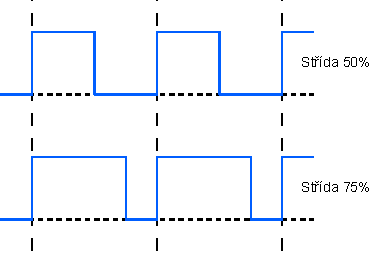
\includegraphics[scale=1]{obrazky-figures/pwm_duty_cycle.pdf}
	\caption{PWM signál pro různé hodnoty střídy}
	\label{}
\end{figure}

Při pohledu na klasický digitální signál který rovnoměrně střídá vysokou a nízkou úroveň by šlo říci, že se jedná o PWM signál se střídou 50\%. Střída (duty cycle) udává poměr času, kdy je signál v logické jedničce, ku času, kdy je v nule. Součet těchto hodnot se musí rovnat délce jedné periody. Úpravou tohoto poměru lze simulovat analogový signál. \cite{embeded_robotics}

\subsection*{I2C}
Je synchronní sběrnice, která se vyznačuje svou jednoduchostí a nízkou cenou. Využívá dva vodiče SDA (serial data) a SCL (serial clock). Oba vodiče jsou připojeny k napájecímu napětí pomocí pull-up rezistoru a bez vlivu jiného hardwaru tedy zůstávají v logické jedničce. Zařízení, která jsou na tuto sběrnici připojeny, využívají open drain k úpravě aktuální napěťové úrovně. I2C pracuje s dvěma druhy zařízení, master a slave. Master zahajuje, řídí a ukončuje komunikaci na vodiči SDA a po dobu průběhu komunikace generuje hodinový signál na SCL. Typicky se jedná o mikrokontroler. Slave jsou pak ostatní zařízení s nimiž může master komunikovat, typicky různé periferie. \cite{embeded_robotics}

\begin{figure}[h!]
	\centering
	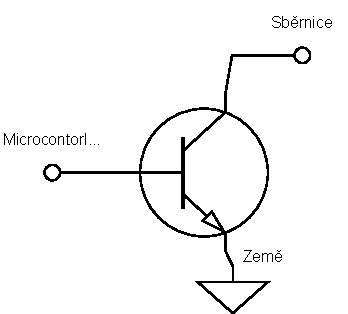
\includegraphics[scale=1]{obrazky-figures/open_drain.pdf}
	\caption{Open drain}
	\label{}
\end{figure}

Přenos jednoho datového rámce zahájí master zařízení přivedením datové sběrnice do nuly. Následující komunikace se skládá z odeslání rámce o délce osmi bitů a potvrzení o úspěšném přenosu dat od přijímajícího zařízení. Toto potvrzení se nazývá ACK a je provedeno podržením datové sběrnice v hodnotě nula po dobu jednoho taktu. Opačný stav se nazývá NACK a indikuje že nastala chyba. Ukončení přenosu je provedeno navrácením datové sběrnice na hodnotu jedna. \cite{um10204}

\begin{figure}[h!]
	\centering
	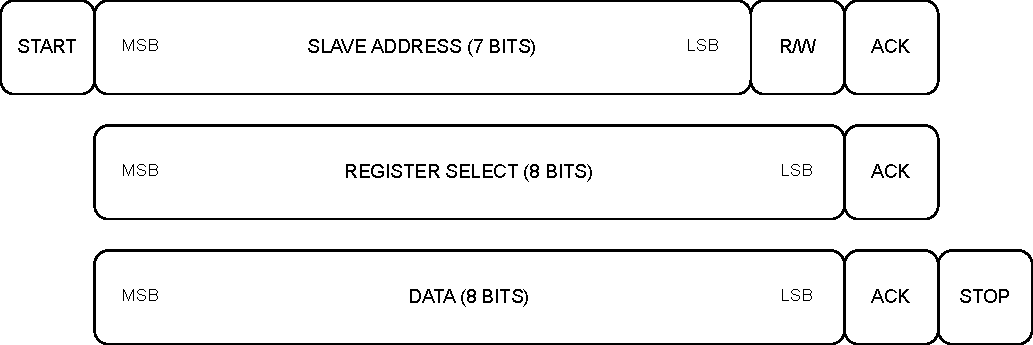
\includegraphics[scale=0.75]{obrazky-figures/i2c_data_word.pdf}
	\caption{Datové slovo sběrnice I2C}
	\label{}
\end{figure}

Na obrázku lze vidět, jak může vypadat přenos jednoho datového slova. V prvním rámci je přenesena sedmi bitová adresa, identifikující slave zařízení se kterým chce máster navázat komunikaci. Osmý bit datového rámce indikuje směr, kterým budou posílány data. V druhém rámci dojde k adresaci konkrétního registru na slave zařízení. A ve třetím, případně dalších, již probíhá samotné posílání dat mezi zařízeními. \cite{an4481}

\section{Adeept AWR 4WD}
Pohyb tohoto robota zajišťují čtyři pevná kola a zatáčení je tedy realizováno diferenciálním způsobem. To znamená, že jednotlivá kola se mohou otáčet svou vlastní rychlostí a zpomalením kol na jedné straně oproti té druhé lze provést zatáčení robota. Velkou výhodou tohoto přístupu je možnost otáčení robota na místě. Nevýhodou pak budou složitější výpočty při potřebě zahnout o nějaký přesně daný úhel.

\noindent Následující stránky popisují jednotlivé komponenty tohoto robota.

\subsection*{Robot HAT}
HAT(hardware attached on top) je hardwarová deska, která slouží k rozšíření mikrokontroléru o další funkcionalitu. Tato konkrétní se k Raspberyy Pi připojuje pomocí GPIO(General purpuse input outpu) pinů. Deska jako taková obsahuje rozšiřující čipy a rozhraní sloužící k ovládání připojených periferií.

\begin{itemize}
	\item{PCA9685 \cite{pca9685}}
	\begin{itemize}
		\item{generátor PWM signálu}
		\item{16 kanálů}
		\item{12 bitů rozlišení střídy (4096 možných hodnot)}
		\item{je ovládaný přes I2C sběrnici}
	\end{itemize}
	\item{L298P \cite{l298}}
	\begin{itemize}
		\item{ovladač pro řízení dc motoru}
		\item{základem je full bridge obvod}
		\item{umožňuje roztočit motor oběma směry}
		\item{pomocí PWM lze ovládat rychlost motorů}
		\item{připojuje motor na externí napájení}
	\end{itemize}
	\item{další rozhraní pro připojení periferií (sledování čáry, ultrazvukový senzor, led)}
\end{itemize}

\begin{figure}[h!]
	\centering
	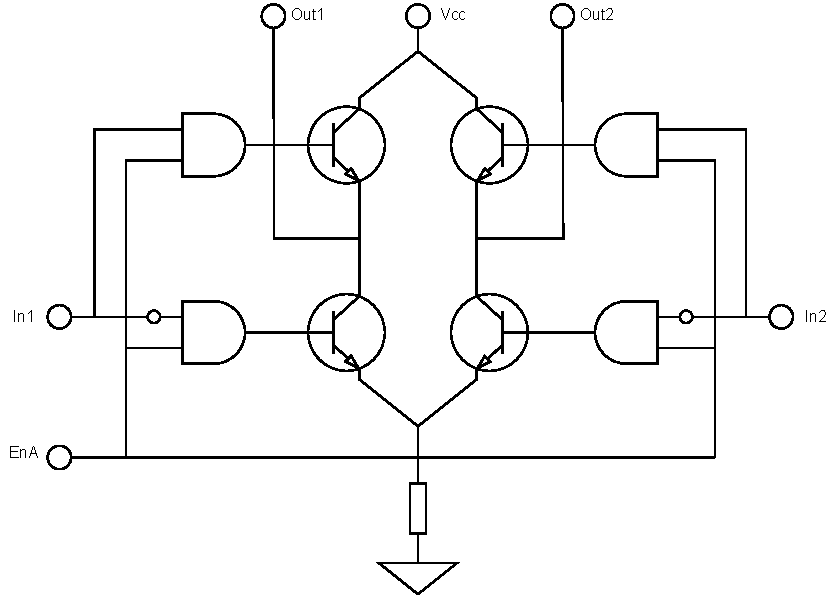
\includegraphics[scale=0.75]{obrazky-figures/motor_full_bridge.pdf}
	\caption[Full bridge ovladač motoru.]{Full bridge konfigurace pro ovládání motoru. In1 a In2 určují směr otáčení. EnA je PWM signál určující rychlost otáčení. \cite{l298}}
	\label{}
\end{figure}

\newpage
\subsection*{DC Motor}
Pohyb celého autíčka zajišťují čtyři stejnosměrným proudem(direct current) napájené motory. Ovladač motorů L298P je umístěný na Robot HAT.

\begin{figure}[h!]
	\centering
	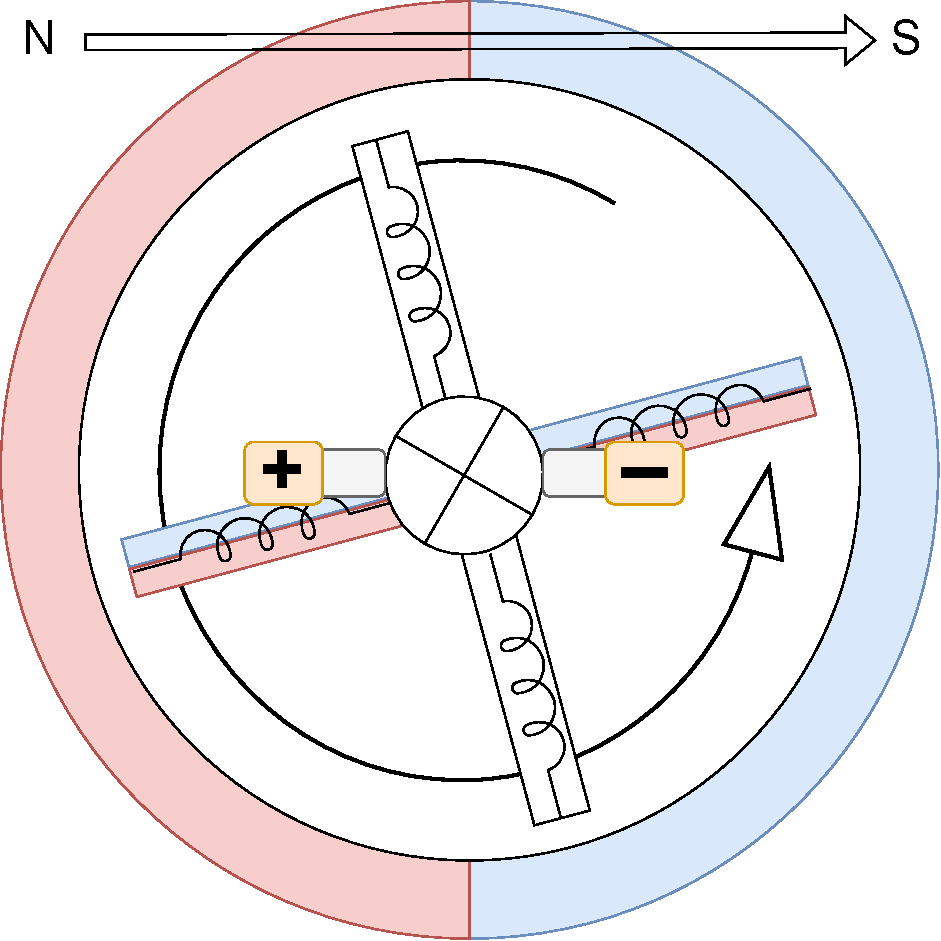
\includegraphics[scale=0.50]{obrazky-figures/dc_motor.pdf}
	\caption{Schéma DC motoru}
	\label{}
\end{figure}

Elektrický DC motor se skládá ze dvou hlavních částí, stator a rotor. Stator je statická, vnější část, a typicky se jedná o permanentní magnet. Uvnitř statoru se pak nachází rotor, ten se skládá z elektromagnetů, které při zapnutí reagují se statorem(opačné póly se přitahují a stejné odpuzují) a dojde tak k částečnému pootočení. Při správném spínání a vypínání těchto elektromagnetů lze motor rozběhnout. 
Toto střídání zajišťuje prstenec zvaný komutátor. Komutátor je rozdělen na několik od sebe odizolovaných částí, ke kterým jsou připojeny vývody elektromagnetů. S povrchem prstence jsou pomocí pružin v kontaktu dva kartáče. Tyto kartáče se již neotáčí a mohou tak být připojeny na zdroj napájení a zem. Komutátor se otáčí společně s rotorem a při tomto pohybu se kartáče postupně dotýkají různých částí komutátoru a spínají tak jednotlivé elektromagnety, ty zajistí pootočení rotoru a sepnutí následujícího magnetu. \cite{dc_motor}

\subsection*{Servo}
Servo je komponenta na první pohled podobná DC Motoru. Na rozdíl od něj se však neotáčí celých 360 stupňů, ale bývá omezena na nějakou menší hodnotu, například 180 stupňů. Hlavním výhodou a důvodem pro použití serva je plná kontrola nad úhlem natočení jeho hřídele. \cite{embeded_robotics}

\begin{figure}[h!]
	\centering
	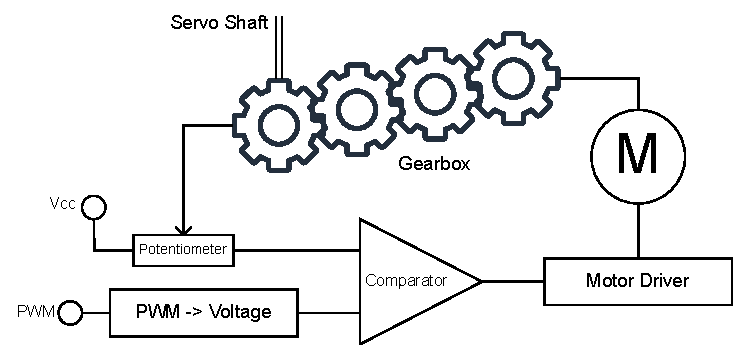
\includegraphics[scale=0.9]{obrazky-figures/servo.pdf}
	\caption{Vnitřní zapojení serva}
	\label{}
\end{figure}

Při pohledu na vnitřní zapojení serva lze zjistit, že se prakticky jedná o klasický dc motor připojený na převodovku a rozšířený o elektroniku na jeho řízení. K nastavení úhlu serva se využívá PWM signál. Ten je první přeložený na napěťovou úroveň, která je porovnána s aktuálním natočením serva a výsledek udává směr, kterým se bude otáčet motor. Aktuální natočení serva je získáno využitím potenciometru zapojeného na výstupní hřídel serva. \cite{embeded_robotics}

\subsection*{Ultrazvukový senzor hloubky} \label{theory:ultrasonic}
Slouží k určení vzdálenosti mezi robotem a překážkou. Funguje na principu radaru. Vyšle ultrazvukovou vlnu na frekvenci 40Khz a uloží si časovou značku. Následně poslouchá než se mu vrátí odražená vlna a opět si uloží značku.
Pro výpočet vzdálenosti lze využít následující vzorec:

$$S = \frac{(T_2 - T_1) * V_S}{2}$$

Kde $T_1$ je moment kdy byla vyslána vlna $T_2$ kdy byla vlna přijata a $V_S$ rychlost šíření zvuku ve vzduchu (cca 340m/s). Výsledek se pak dělí dvěma, protože doba $T_2 - T_1$ je rovna času k překážce a zpět.

Ovládání senzoru je pak realizováno pomocí dvou jeho vývodů, trig a echo. Mikrokontroler vyšle pulz na trig vodiči. Ten zaktivuje senzor, který zahájí měření. To je realizováno osmi čtyřicetihercovými pulzy. Po dokončení měření nastaví echo vodič do hodnoty jedna na dobu rovnou času mezi odesláním a zachycením ultrazvukového signálu. \cite{embeded_robotics}

\begin{figure}[h!]
	\centering
	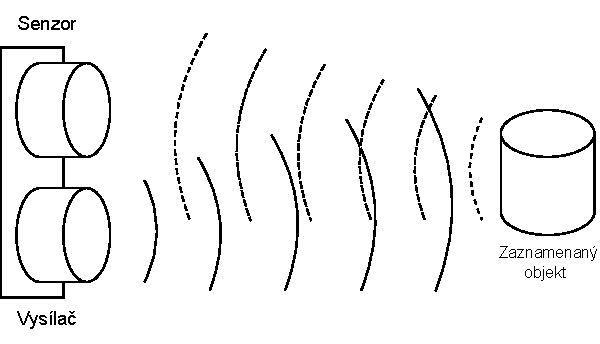
\includegraphics[scale=0.75]{obrazky-figures/ultrasonic.pdf}
	\caption{Ultrazvukový senzor}
	\label{}
\end{figure}

\subsection*{Třícestný senzor pro sledování čáry}
Modul využívá fakt, zě intenzita světla odraženého od povrchu je závislá na barvě dané plochy. Například černá barva pohltí téměř veškeré světlo, naopak bílá téměř vše odrazí. Používáno je infračervené záření, protože není ovlivněno okolními zdroji světla, odráží se od velkého množství materiálů a je přesné. Jedná se o třícestný modul a skládá se tedy ze setu tří vysílačů a senzorů. Pokud vysílač svítí a senzor nezaznamenává dostatečnou intenzitu odraženého světla, znamená to, že byla nalezena černá čára. \cite{embeded_robotics}

\subsection*{WS2812 RGB LED}
WS2812 je druh adresovatelných LED diod. Pojmem adresovatelných je myšleno, že není každá dioda připojena k mikrokontroleru zvláště, ale sdílejí jeden datový vodič pro nastavování barev. Prakticky to znamená, že pásek, který může obsahovat i stovky diod je připojený jen pomocí tří vodičů. Těmito vodiči jsou napájení, země a vstupní data. \cite{ws2812}

\begin{figure}[h!]
	\centering
	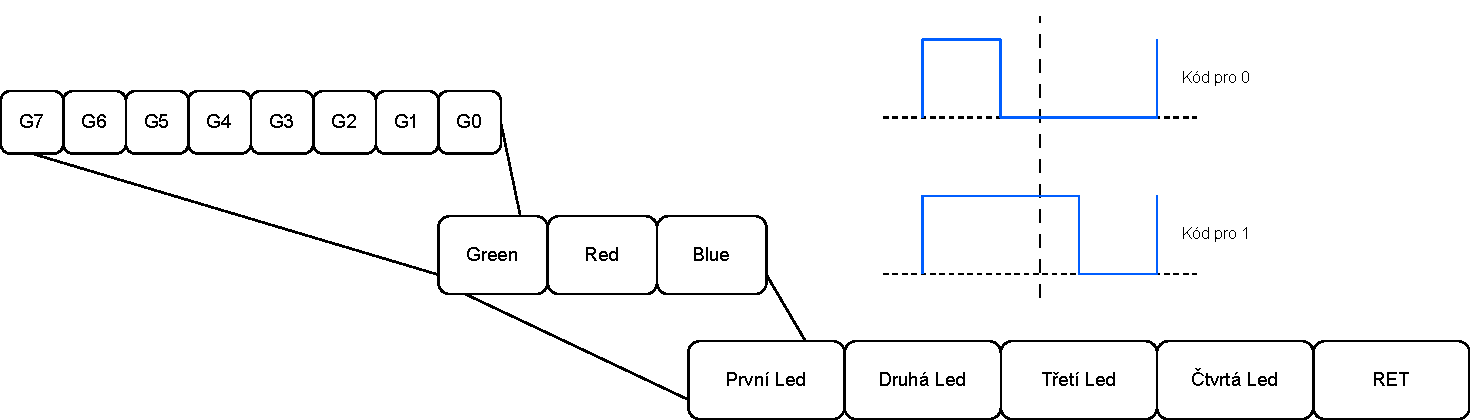
\includegraphics[scale=0.55]{obrazky-figures/ws2812_led.pdf}
	\caption{Komunikační protokol pro WS2812 led}
	\label{}
\end{figure}

Diody jsou na pásku zapojeny sériově. Každá dioda má DIN a DO port. Pokud dioda přijme data, která jí nejsou určená, přeposílá je dále. Komunikace vždy začíná klidovým stavem, datový vodič je v nule. Datové slovo se skládá z 24 bitových bloků pro každou diodu. Blok obsahuje tři osmi bitové hodnoty, jednu pro každou barevnou složku (MSB je posíláno první). Diody pak fungují tak, že přijmou prvních 24 bitů, podle kterých nastaví svou barvu. Tuto část odeberou z datového slova a zbytek přeposílají na výstup. \cite{ws2812}

\section{Rozšíření Hardware komponent}

\subsection*{Lidar}
Jedná se o senzor sloužící k měření vzdálenosti. Narozdíl od sonaru nebo radaru však využívá k tomuto účelu světlo a konkrétně laser. 

\subsection*{Inertial Mesurement Unit}
Jedná se o senzor sloužící k měření a určení pozice a orientace. Konkrétní použitý IMU senzor disponuje tříosým gyroskopem a akcelerometrem. 

\subsubsection*{MEMS}
Což znamená micro-electromechanical systems. Jak z názvu vyplývá jedná se o systémy využívající mechanické elementy ve velikostech typických pro elektronické součástky. Typicky se jedná o velikosti pod 100$\mu m$.

\subsubsection*{Princip Akcelerometru}
Akcelerometr na čipu je postavený na principu MEMS. 

\begin{figure}[h!]
	\centering
	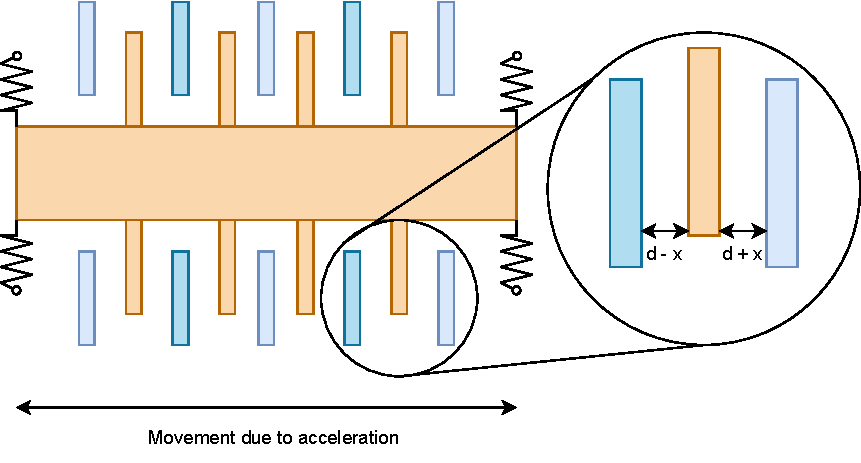
\includegraphics[scale=0.8]{obrazky-figures/accelerometer.pdf}
	\caption{Struktura akcelerometru}
	\label{}
\end{figure}

Senzor pak funguje na tom principu, že střední část umístěná na pružinách má nějakou nezanedbatelnou váhu a vnější akcelerace tak způsobí pohyb relativně ke zbytku systému. Jak na pohyblivé tak na statické části se pak nachází desky tvořící části kondenzátoru. Pohyb střední části způsobí změnu kapacity těchto kondenzátorů kterou lze měřit.

Základní rovnice pro výpočet kapacity je následující:
$$C = \epsilon \frac{A}{d}$$
Kde $C$ je výsledná kapacita $\epsilon$ je $A$ plocha desek $\epsilon$ permitivita prostředí mezi nimi a $d$ jejich vzdálenost.

Statické desky jsou zapojeny střídavě a rozdíl mezi jejich kapacitami pak odpovídá posunutí vnitřní části.
$$x \approx d \frac{\Delta C}{C_0}$$

\subsubsection{Princip Gyroskopu}
Gyroskop na čipu je využívá podobné principy jako akcelerometr. Skládá se ze dvou částí, vnitřní a vnější (senzorický) rám. Ve vnitřním rámu je umístěná pohyblivá část s nezanedbatelnou hmotností. Na rozdíl od akcelerometru není tato část v klidovém stavu statická ale je rozvibrována do harmonické oscilace podél osy x.
Vnitřní rám je celý umístěn pohyblivě, pomocí pružin, uvnitř senzorického rámu. Při rotaci gyroskopu se bude vnitřní oscilující část snažit držet původní směr, ve kterém se pohybovala, což způsobí pohyb celého vnitřního rámu podél osy y. Tento pohyb je pak detekován pomocí změn kapacit kondenzátorů, stejně jako u akcelerometru. 

\begin{figure}[h!]
	\centering
	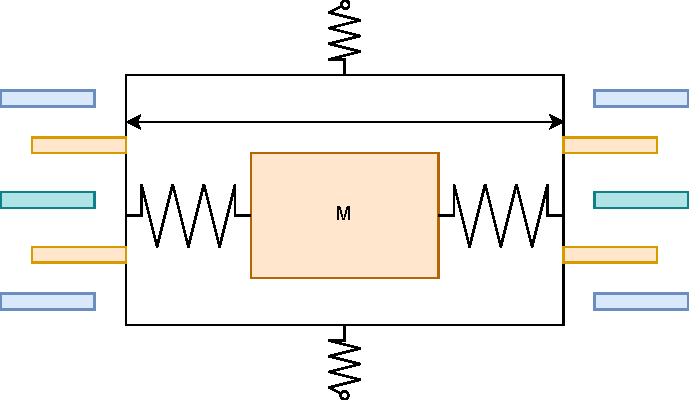
\includegraphics[scale=0.8]{obrazky-figures/gyroscope.pdf}
	\caption{Struktura akcelerometru}
	\label{}
\end{figure}

\section{Raspberry Pi 4b}
Jako mozek celého systému je použit mikropočítač Raspberry Pi. V porovnání s běžně používanými mikrokontroléry, sloužícími pro řízení vestavěných systémů, se jedná o výkonnější hardware, který zvládá i komplexnější operace, jako běh plnohodnotného operačního systému a zpracování obrazu. Konkrétně se jedná o verzi 4 model B s operační pamětí o velikosti čtyř gigabajtů. Tato verze obsahuje 64bitový procesor, ten je potřeba pro spuštění 64 bitového Ubuntu serveru, který je doporučeným operačním systémem pro požití ROS2 na Raspberry Pi.
Komunikace s většinou použitých periferií je uskutečněna pomocí General Purpuse Input Output(GPIO) pinů. Jedná se o číslicové vývody, které podle potřeby můžou fungovat jako vstup i výstup ze zařízení. Některé z nich pak mají ještě speciální funkce, například GPIO 2 a 3 můžou pracovat jako SDA a SCL připojení pro I2C komunikaci.

\begin{figure}[h!]
	\centering
	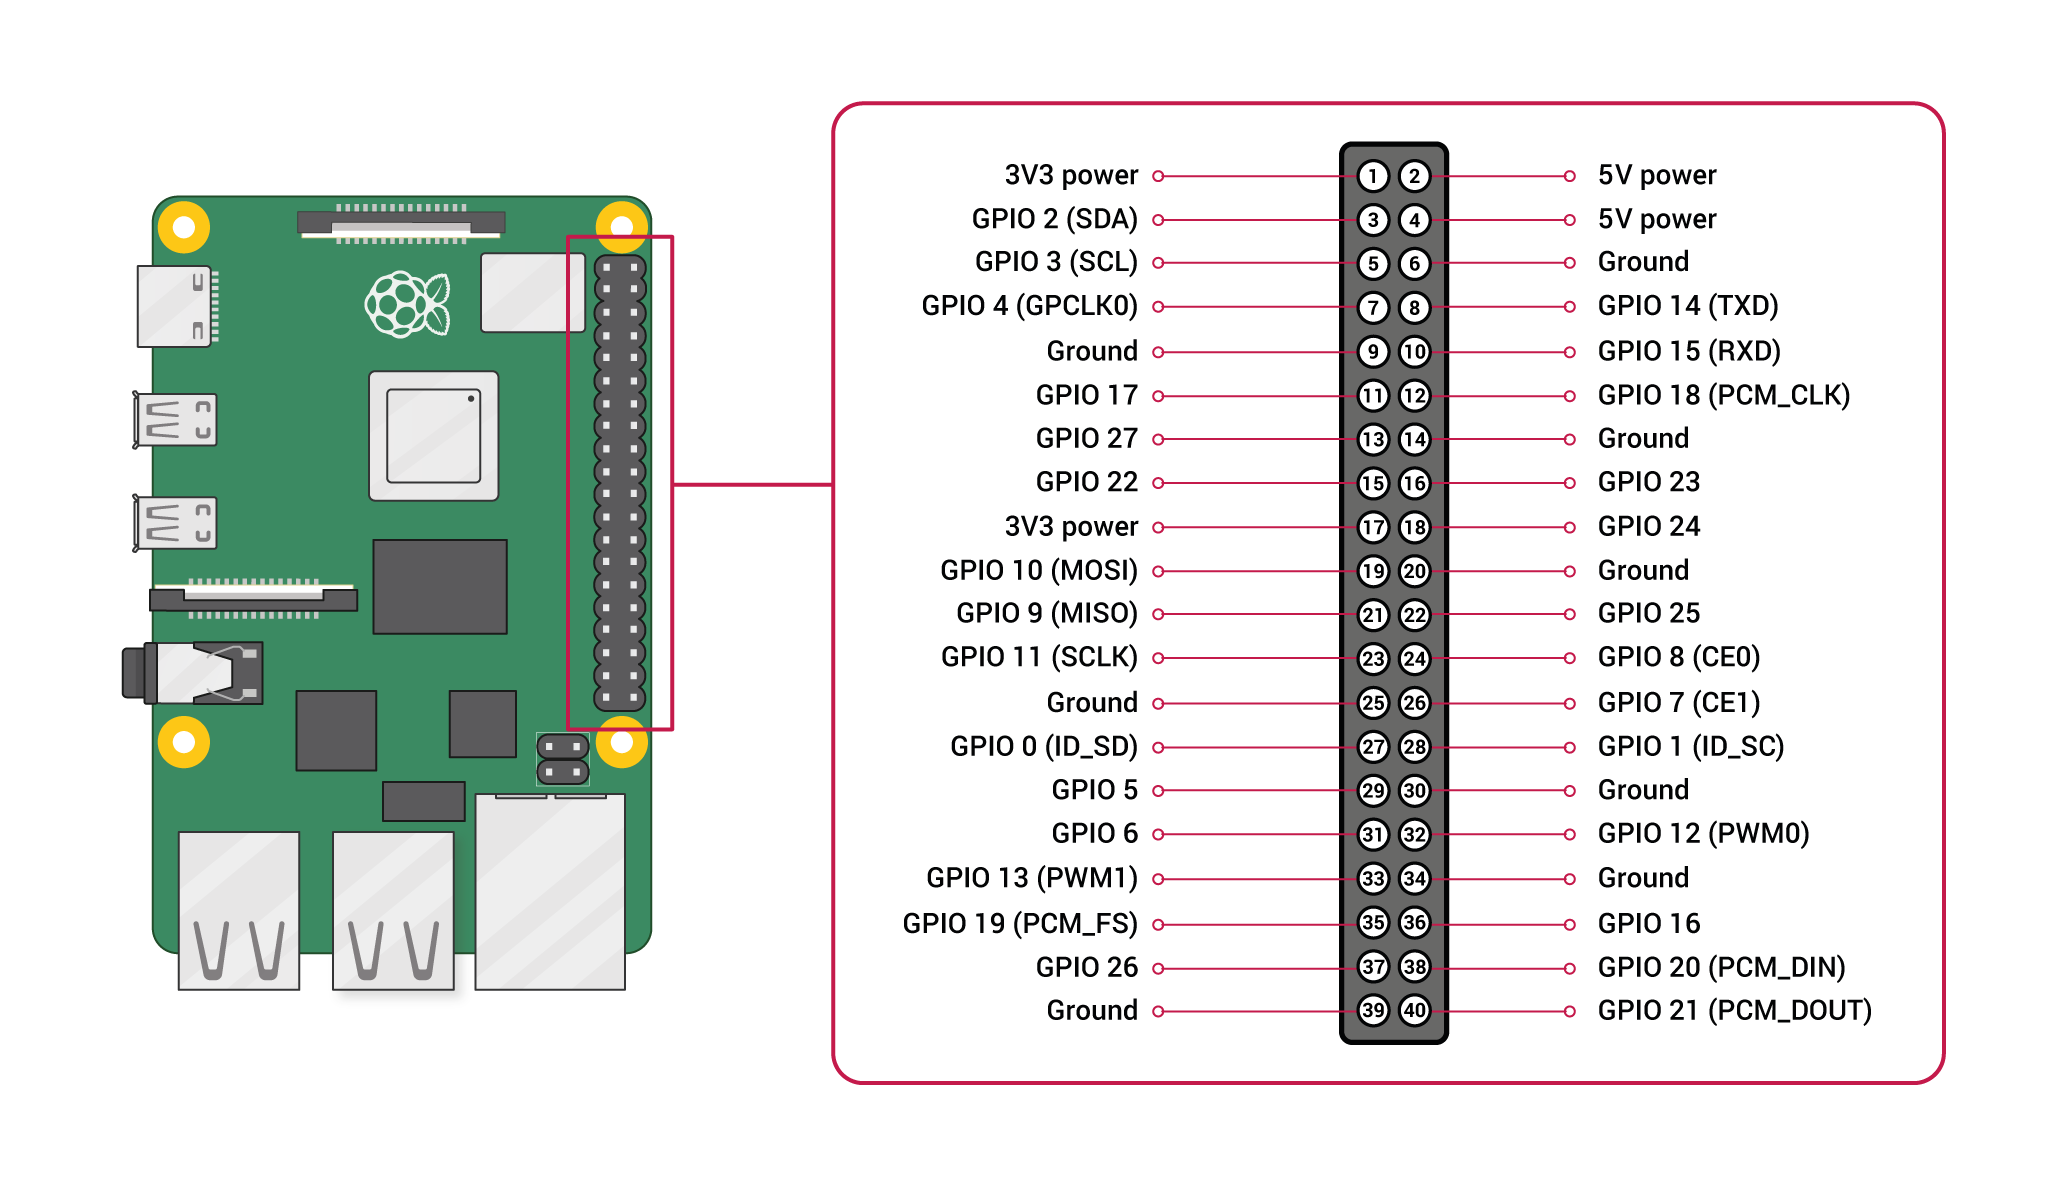
\includegraphics[scale=0.15]{obrazky-figures/gpio_pinout.png}
	\caption{GPIO pinout pro Raspberry Pi}
	\label{}
\end{figure}

\subsection*{Camera}
Přímo k rapsberry pi je připojena oficiální rpi camera v3. Tento modul dokáže nahrávat video až v rozlišení 2304 × 1296 pixelů a 56 snímcích za vteřinu. Avšak pro zpracování, případně analýzu obsahu videa v reálném čase s těmito specifikacemi nemá Raspberry Pi dostatečný výkon. Prakticky budou využity nižší rozlišení a snímkovací frekvence. \cite{rpi_camera}
%opencv

\chapter{Software pro řízení robota}
Jak už bylo řečeno, software poběží na Raspberry Pi. Jako primární programovací jazyk byl zvolen python, protože je jedním z oficiálních jazyků podporovaných ROS2 a také jsou v něm implementovány potřebné knihovny pro ovládání periferií.

\section{Aktuální software}
Robot Adeept AWR 4WD je dodáván s ukázkovým softwarem. Ten je implementován v jazyce Python a využívá knihovny třetích stran sloužící k nízkoúrovňovému ovládání hardwarových komponent. Aby byl robot responzivní je celá implementace řešena s použitím python modulů pro realizaci multithreadingu.

\section{Seznámení s ROS2}
ROS2 je middleware sloužící k vývoji a řízení robotů. Middleware je softwarová vrstva běžící nad operačním systémem. Jejím úkolem je rozšíření operačního systému o další funkcionalitu. Typickou součástí middlewaru bývají knihovny, ovladače, vývojové a monitorovací nástroje. Může také specifikovat doporučené metodologie pro vývoj. ROS2 je již druhá verze tohoto softwaru, která rozšiřuje a opravuje neduhy první verze. Původní ROS1 je považován za de-facto standart pro vývoj robotických aplikací.
Tato práce využívá ROS2 distribuci jménem iron. Distribuce v ROS2 lze popsat jako set operačního systému, knihoven a dalších aplikací, které jsou otestovány a je zaručeno, že jsou navzájem kompatibilní. Velkou výhodou ROS je fakt, že se jedná o open source projekt. Díky tomu kolem něj vznikla velká komunita vývojářů, ale i firem a dalších institucí, které tvoří mnoho souvisejícího obsahu. Existuje tedy velké množství knihoven, dokumentací a návodů které usnadňují vývojářům práci. \cite{ros2_introduction}

\subsection*{Vrstvy ROS2}
Na nejvyšší úrovni, se nachází programátor, který interaguje s klientskými knihovnami pro vývoj ROS2 aplikací. Tyto knihovny jsou oficiálně dvě a to rclpy pro python a rclcpp pro C++. Existují také implementace pro další programovací jazyky (rclc, java, C\#), které jsou však udržovány komunitně. Všechny klientské knihovny pak využívají RCL. To je jádrem celého ROS a obsahuje implementaci všech ROS2 funkcionalit. Je napsáno v jazyce C a jeho součástí je rozhraní, pomocí kterého poskytuje svou funkcionalitu ostatním klientským knihovnám. Díky tomuto přístupu se uzly implementované v pythonu budou chovat stejně jako ty implementované v c++. Z toho pak také vyplývá, že uzly implementované na různých klientských knihovnách spolu mohou bez problémů komunikovat.
Poslední vrstvou je data distribution service. DDS je komunikační vrstva implementována na UDP protokolu sloužící k předávání informací mezi procesy. Má charakteristiky systémů reálného času, zajišťuje kvalitu a zabezpečení komunikace. Také umožňuje vyhledávání uzlů bez potřeby centralizovaného serveru (vyhledávání je realizováno s využitím multicastové komunikace, zprávy zasílané mezi jednotlivými uzly pak využívají klasický unicast). \cite{ros2_introduction}

\begin{figure}[h!]
	\centering
	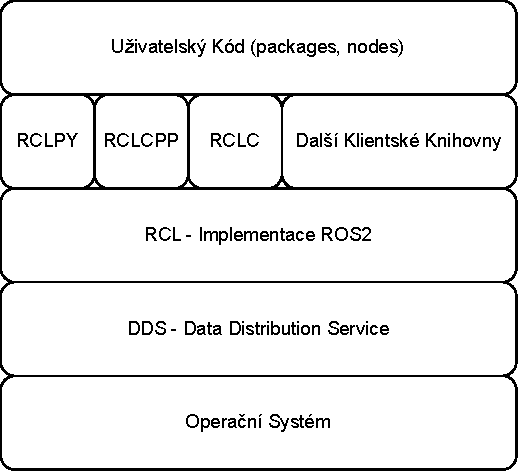
\includegraphics[scale=0.75]{obrazky-figures/ros_layers.pdf}
	\caption{Vrstvy ROS2 systému}
	\label{}
\end{figure}

\subsection*{Vývoj v ROS2}
Nejvyšší organizační jednotkou v ROS2 je workspace. Jedná se o složku, která slouží k organizaci zdrojových souborů, jejich instalaci a následné spouštění. ROS2 se také kvalifikuje jako workspace a před použitím musí být nejprve aktivován. K tomu v linuxu slouží příkaz \verb|source|. Aktivace workspace je akumulativní, to znamená, že v jeden moment může být aktivních několik workspace najednou. Typicky se první aktivuje základní ROS2 instalace, která tvoří takzvanou underlay vrstvu. Vývojový workspace aktivovaný jako druhý, se pak nazývá overlay. Pokud má overlay nějaké závislosti, měly by být uspokojeny v underlay.
Zdrojové soubory v rámci workspace jsou pak organizovány do packages. Package může obsahovat zdrojové soubory, knihovny a definice zpráv. Packages na sobě můžou navzájem záviset (např: package která využívá interface závisí na jiné která tento interface definuje). \cite{ros2_introduction}

\begin{figure}[h]
	\begin{forest}
		for tree={
			font=\ttfamily,
			grow'=0,
			child anchor=west,
			parent anchor=south,
			anchor=west,
			calign=first,
			inner xsep=7pt,
			edge path={
				\noexpand\path [draw, \forestoption{edge}] (!u.south west) +(7.5pt,0) |- (.child anchor) \forestoption{edge label};
			},
			before typesetting nodes={
				if n=1
				{insert before={[,phantom]}}
				{}
			},
			fit=band,
			before computing xy={l=15pt},
		}
		[Workspace
			[build {\hspace{3em}\#soubory používané při kompilaci}
			]
			[install {\hspace{2em}\#výsledky kompilace a další soubory potřebné ke spuštění}
			]
			[log {\hspace{4em}\#logy z kompilace}
			]
			[launch {\hspace{2.5em}\#launch soubory}
			]
			[src {\hspace{4em}\#packages}
				[package\_name {\hspace{2em}\#příklad jak vypadá python package}
					[package\_name {\hspace{2em}\#zdrojové python soubory}
					]
					[resource
					]
					[test
					]
					[package.xml {\hspace{1em}\#metadata infromace o package}]
					[setup.cfg {\hspace{2em}\#konfigurace pro manuální spouštění uzlu}]
					[setup.py {\hspace{2.5em}\#instrukce pro kompilátor jak nainstalovat package}]
				]
			]
		]
	\end{forest}
  	\caption{Struktura ROS2 Workspace}
	\label{}
\end{figure}

\subsubsection*{Node}
Celý ROS2 systém je složený z uzlů (node), které mezi sebou navzájem komunikují. Každý uzel je vlastní výpočetní jednotka, která by měla plnit jeden specifický úkol. Tento přístup je podobný objektově orientovanému návrhu a ROS2 jej také využívá. Implementačně je uzel objekt, který dědí ze třídy \verb|Node|.
Uzly v ROS2 většinou nepotřebují běžet permanentně, ale pouze v monentě, kdy nastane nějaká událost, kterou je potřeba obsloužit. Z toho důvodu existuje v ROS2 metoda \verb|spin()|, která uspí vykonávání uzlu, dokud jej není potřeba opět využít. Aby ROS2 šetřil výpočetní prostředky, využívá dva přístupy k určení, kdy bude potřeba uzel vzbudit. Prvním je iterative execution, ten se používá u uzlů, které vykonávájí svou činnost pravidelně na nějaké předem dané frekvenci. Například se může jednat o výpočetní uzel, který pravidelně každých x mikrosekund provede výpočet podle hodnot senzorů a odešle výsledek.
Druhý je event oriented execution. Zde dochází k vyvolání řídícího cyklu jako důsledek nějaké události, typicky se jedná od příchozí zprávu z subscription, service nebo action. Frekvenci spouštění těchto uzlů pak lze odvodit od frekvence příchozích zpráv. Typicky se může jednat o uzel přijímající snímky z kamery na kterých provede výpočet a vrátí odpověď. Frekvence výpočtu je dána příchozími snímky, pokud snímky přestanou přicházet, uzel se nebude spouštět. \cite{ros2_introduction} \cite{ros2_documentation}

\begin{algorithm}[h!]
	\label{}
	\caption{\textsc{Definice a použití Node objektu}}
	
	\DontPrintSemicolon
	\SetAlgoNoLine
	\SetAlgoNlRelativeSize{-1}
	\SetNlSty{}{}{:}
	\SetNlSkip{-1.1em}
	
	\BlankLine \Indp\Indpp
	
	\texttt{class CustomNode(Node):}\;
	\Indp\Indp
	\texttt{def \_\_init\_\_(self):}\;
	\Indp\Indp
	\texttt{super().\_\_init\_\_('node\_name')}\;
	\Indm\Indm\Indm\Indm
	
	\BlankLine
	
	\texttt{def main(args):}\;
	\Indp\Indp
	\texttt{rclpy.init(args=args)}\;
	\texttt{node = CustomNode()}\;
	\texttt{rclpy.spin(node)}\;
	\texttt{node.destroy\_node()}\;
	\texttt{rclpy.shutdown()}\;
\end{algorithm}

\subsubsection*{Topic}
Je základním a také nejčastěji používaným způsobem pomocí kterého spolu ROS2 uzly komunikují. Topic si lze představit jako analogii hardwarové sběrnice. Prakticky se jedná o přesně pojmenované místo, do kterého může n uzlů posílat data (Publish) a m poslouchat co bylo posláno (Subscribe). Zprávy posílané do topicu mají přesný formát a jsou posílány asynchronně. Příkladem použití může být topic, do nějž posílá data uzel ovládající kameru a několik dalších uzlů které tyto data potřebují jej mohou číst. \cite{ros2_introduction}

\begin{algorithm}[h!]
	\label{}
	\caption{\textsc{Subsrciber Node}}
	
	\DontPrintSemicolon
	\SetAlgoNoLine
	\SetAlgoNlRelativeSize{-1}
	\SetNlSty{}{}{:}
	\SetNlSkip{-1.1em}
	
	\BlankLine \Indp\Indpp
	\texttt{self.create\_subscription(Interface, "topic\_name", self.callback\_function, queue\_size)}\;
	
	\BlankLine
	\texttt{def callback\_function(self, msg):}\;
	\Indp\Indp
	\texttt{value = msg.item}\;
\end{algorithm}
Tento kód ukazuje, jak se může uzel přihlásit v odebírání zpráv z topicku. Nejprve je potřeba (typicky v konstruktoru třídy) zavolat zděděnou metodu sloužící k inicializaci nějaké ROS2 funkcionality. V tomto případě se jedná o \verb|create_subscription|. Jako parametry potřebuje jméno, interface, callback funkci a délku fronty. Inteface definuje formát zpráv a délka fronty je použita v případě, že uzel nezvládá přijímat zprávy dostatečně rychle. Callback funkce je pak zavolána pokaždé když do topicku přijde nová zpráva. Druhým parametrem callback funkce je předán objekt, který ve svých atributech obsahuje hodnoty dané zprávy. \cite{ros2_documentation}

\begin{algorithm}[h!]
	\label{}
	\caption{\textsc{Publisher Node}}
	
	\DontPrintSemicolon
	\SetAlgoNoLine
	\SetAlgoNlRelativeSize{-1}
	\SetNlSty{}{}{:}
	\SetNlSkip{-1.1em}
	
	\BlankLine \Indp\Indpp
	\texttt{self.publisher = self.create\_publisher(Interface, "topic\_name", queue\_size)}\;
	
	\BlankLine
	\texttt{output = Interface()}\;
	\texttt{output.item = some\_value}\;
	\texttt{self.publisher.publish(output)}\;
\end{algorithm}
Odesílání zpráv do topicu demonstruje tento kód. Jeho struktura je podobná předchozímu příkladu. Odeslání zprávy demonstrují řádky 2--4. Nejprve dojde k inicializaci objektu interface, stejného datového typu jako ten, který používá topic. Tento objekt je následně naplněn daty a pomocí metody \verb|publish()| předem vytvořeného publisheru odeslán. \cite{ros2_documentation}

\subsubsection*{Service}
Sevice funguje na stejném principu jako klient--server komunikace známá z počítačových sítí. Jedná se tedy o synchronní komunikaci, kde jeden uzel poskytuje nějakou službu a ostatní si na ni mohou poslat požadavek. Od service uzlu se typicky předpokládá okamžitá odpověď, aby nedošlo k narušení řídícího cyklu volajícího uzlu. \cite{ros2_introduction}
\newpage

\begin{algorithm}[h!]
	\label{}
	\caption{\textsc{Service server}}
	
	\DontPrintSemicolon
	\SetAlgoNoLine
	\SetAlgoNlRelativeSize{-1}
	\SetNlSty{}{}{:}
	\SetNlSkip{-1.1em}
	
	\BlankLine \Indp\Indpp
	
	\texttt{self.srv = self.create\_service(Interface, "service\_name", self.callback\_function)}\;
	\BlankLine
	\texttt{def callback\_function(self, request, response):}\;
	\Indp\Indp
	\texttt{value = request.item}\;
	\texttt{response.item = some\_value}\;
	\texttt{return response}\;
	
\end{algorithm}
Změnou oproti předchozím příkladům je přidání nového parametru do callback funkce. Tato funkce má nyní dva důležité parametry, request a response. Request obsahuje konkrétní hodnoty požadavku na server a response je potřeba naplnit výsledky a vrátit z funkce. \cite{ros2_documentation}

\begin{algorithm}[h!]
	\label{}
	\caption{\textsc{Service client}}
	
	\DontPrintSemicolon
	\SetAlgoNoLine
	\SetAlgoNlRelativeSize{-1}
	\SetNlSty{}{}{:}
	\SetNlSkip{-1.1em}
	
	\BlankLine \Indp\Indpp
	
	\texttt{self.cli = self.create\_client(Interface, "service\_name")}\;
	\texttt{while not self.cli.wait\_for\_service(timeout\_sec=1.0):}\;
	\Indp\Indp
	\texttt{pass}\;
	\Indm\Indm

	\BlankLine
	\texttt{def send\_request(self):}\;
	\Indp\Indp
	\texttt{self.req = Interface.Request()}\;
	\texttt{self.req.item = some\_value}\;
	\texttt{self.future = self.cli.call\_async(self.req)}\;
	\texttt{rclpy.spin\_until\_future\_complete(self, self.future)}\;
	
	\BlankLine
	\texttt{response = self.future.result()}\;
	\texttt{value = response.item}\;
\end{algorithm}
Service client narozdíl od topic subscriberu závisí na tom, aby existoval server, který je schopný odpovídat na jeho požadavky. Tato podmínka vyplývá z faktu, že service server by měl odpovídat na dotazy téměř okamžitě a service klient tedy předpokládá, že vždy dostane odpověď. Pokud by neexistoval server, klient by při požadavku skončil v nekonečném čekání. Proto je hned v konstruktoru implementována kontrola, které nedovolí vytvoření uzlu dokud není přítomen server. Čekání na odpověď od serveru, je pak implementována pomocí funkce \verb|spin_until_future_complete()| \cite{ros2_documentation}

\subsubsection*{Action} %cite web documentation
Jedná se o rozšířenou verzi service. Akce z pravidla vykonává déle trvající požadavek. Například provedení řídícího manévru robota, který je prováděn v reálném světě a z pohledu uzlu se nejedná o krátkodobou záležitost. Akce, na rozdíl od service, dokáže v průběhu vykonávání své činnosti odesílat průběžné aktualizace o aktuálním stavu zpět volajícímu uzlu. Implementačně akce funguje jako dva service a jeden topic. Cílový (goal) service slouží k zaslání požadavku na server a jeho potvrzení. Výsledkový (result) pak vrací výsledek operace. V průběhu akce pak server posílá aktualizace do topicu. \cite{ros2_introduction}
\newpage

\begin{algorithm}[h!]
	\label{}
	\caption{\textsc{Action server}}
	
	\DontPrintSemicolon
	\SetAlgoNoLine
	\SetAlgoNlRelativeSize{-1}
	\SetNlSty{}{}{:}
	\SetNlSkip{-1.1em}
	
	\BlankLine \Indp\Indpp
	
	\texttt{self.action\_server = ActionServer(self, Interface, "action\_name", self.callback\_function)}\;
	
	\BlankLine
	\texttt{def callback\_function(self, goal\_handle):}\;
	\Indp\Indp
	\texttt{goal\_handle.request.item}\;
	
	\BlankLine
	\tcp{odeslání zpětné vazby volajícímu}
	\texttt{feedback = Interface.Feedback()}\;
	\texttt{feedback.item = some\_value}\;
	\texttt{goal\_handle.publish\_feedback(feedback)}\;
	
	\BlankLine
	\tcp{úspěšné ukončení požadavku}
	\texttt{goal\_handle.succeed()}\;
	\texttt{result = Interface.Result()}\;
	\texttt{result.item = some\_value}\;
	\texttt{return result}\;
\end{algorithm}
Action server využívá stejné postupy jako předchozí ukázky, pouze jich kombinuje více dohromady. V rámci callback funkce může odesílat průběžně zpětnou vazbu a nakonec jako návrat z funkce předá výsledek. \cite{ros2_documentation}

\begin{algorithm}[h!]
	\label{}
	\caption{\textsc{Action client - zaslání požadavku}}
	
	\DontPrintSemicolon
	\SetAlgoNoLine
	\SetAlgoNlRelativeSize{-1}
	\SetNlSty{}{}{:}
	\SetNlSkip{-1.1em}
	
	\BlankLine \Indp\Indpp
	
 	\texttt{self.action\_client = ActionClient(self, Interface, "action\_name")}\;
 	
 	\BlankLine
 	\texttt{def send\_goal(self):}\;
 	\Indp\Indp
 	\texttt{goal\_msg = Servo.Goal()}\;
 	\texttt{goal\_msg.item = some\_value}\;
 	\texttt{self.action\_client.wait\_for\_server()}\;
 	\texttt{self.goal\_future = self.action\_client.send\_goal\_async(goal\_msg, self.feedback\_callback\_function)}\;
 	\texttt{self.goal\_future.add\_done\_callback(self.response\_callback\_function)}\;
	\Indm\Indm
    
\end{algorithm}
Při pohledu na implementaci action klienta lze dobře vidět vnitřní implementace akcí. První funkce \verb|send_goal()| vypadá podobně jako service client. Dojde zde k zaslání požadavku na server a následné čekání na odpověď. Čekání tentokrát není aktivní, aby nedošlo k uváznutí, ale je realizováno pomocí callback funkce. Součástí dotazu je také topic pro zasílání aktualizací. \cite{ros2_documentation}
\newpage

\begin{algorithm}[h!]
	\label{}
	\caption{\textsc{Action client - reakce na přijmutí nebo zamítnutí požadavku}}
	
	\DontPrintSemicolon
	\SetAlgoNoLine
	\SetAlgoNlRelativeSize{-1}
	\SetNlSty{}{}{:}
	\SetNlSkip{-1.1em}
	
	\BlankLine \Indp\Indpp
	
	\texttt{def response\_callback\_function(self, future):}\;
	\Indp\Indp
	\texttt{goal\_handle = future.result()}\;
	\texttt{if not goal\_handle.accepted:}\;
	\Indp\Indp
	\texttt{return}\;
	\Indm\Indm
	
	\BlankLine
	\texttt{self.result\_future = goal\_handle.get\_result\_async()}\;
	\texttt{self.result\_future.add\_done\_callback(self.result\_callback\_function)}\;
	\Indm\Indm
	
\end{algorithm}
Druhá \verb|response_callback_function| pak zpracuje výsledek požadavku (přijmutí nebo zamítnutí) a pošle požadavek na result service, který nakonec vrátí výsledek. \cite{ros2_documentation}

\begin{algorithm}[h!]
	\label{}
	\caption{\textsc{Action client - callback funkce}}
	
	\DontPrintSemicolon
	\SetAlgoNoLine
	\SetAlgoNlRelativeSize{-1}
	\SetNlSty{}{}{:}
	\SetNlSkip{-1.1em}
	
	\BlankLine \Indp\Indpp
	
	\BlankLine
	\texttt{def feedback\_callback\_function(self, msg):}\;
	\Indp\Indp
	\texttt{feedback = msg.feedback}\;
	\texttt{value = feedback.item}\;
	\Indm\Indm
	
	\BlankLine
	\texttt{def result\_callback\_function(self, future):}\;
	\Indp\Indp
	\texttt{result = future.result().result}\;
	\texttt{value = result.item}\;
	
\end{algorithm}

\subsubsection*{Interface}
Interface slouží k určení přesného formátu jednotlivých zpráv, které jsou posílány mezi uzly. ROS2 obsahuje mnoho již vytvořených a vývojáři po celém světě používaných formátů. Tento přístup podporuje znovupoužitelnost vytvořeného kódu a šetří práci. Díky tomu může být software pro ovládání konkrétního kusu hardware naimplementován pouze jednou s využitím standartního rozhraní a všichni ostatní jej pak mohou využít ve svých systémech.
Pokud však standartní interface nevyhovuje potřebám, lze si naimplementovat vlastní. K definici konkrétního formátu slouži tři druhy souborů. \cite{ros2_introduction}

Prvním jsou \verb|.msg| zprávy. Tento formát je využívám topicy. Jedná se o seznam, kde je každá položka definována jako dvojice datový typ a název (případně komentář).
\begin{verbatim}
	int32 angle #comment
	string direction
\end{verbatim}

Druhým je \verb|.srv|. Slouží pro definici request/response zpráv pro komunikaci se servicem. Tento soubor obsahuje dvě části, požadavek a odpověď, každá je tvořena seznamem položek a jsou odděleny řádkem \verb|---|. 
\begin{verbatim}
	int32 a
	int32 b
	---
	int64 sum
\end{verbatim}

Poslední je \verb|.action| soubor. Slouží pro komunikaci s action serverem. Definice se skládá ze tří seznamů, jeden pro požadavek, druhý pro odpověď a poslední pro stavové aktualizace.
\begin{verbatim}
	float32 goal_angle
	---
	bool response
	---
	float32 current_angle
\end{verbatim}

\subsubsection*{Parametry}
ROS2 uzly lze spouštět s parametry. Typicky slouží k nastavení hodnot (předání konfiguračního souboru) za běhu programu bez potřeby zásahu do zdrojových kódů. Příkladem může uzel, sloužící k obsluze periferního zařízení a parametrem jsou mu předány čísla GPIO pinů na které je dané zařízení připojeno. \cite{ros2_introduction}

\begin{algorithm}[h!]
	\label{}
	\caption{\textsc{Parameters}}
	
	\DontPrintSemicolon
	\SetAlgoNoLine
	\SetAlgoNlRelativeSize{-1}
	\SetNlSty{}{}{:}
	\SetNlSkip{-1.1em}
	
	\BlankLine \Indp\Indpp
	
	\tcp{deklarace parametru, typicky v konstruktoru}
    \texttt{self.declare\_parameter('parameter\_name', 'default\_parameter\_value')}\;
	
	\BlankLine
	\tcp{získání hodnoty parametru}
	\texttt{param = self.get\_parameter('parameter\_name').get\_parameter\_value().string\_value}\;
	
	\BlankLine
	\tcp{nastavení hodnoty parametru}
	\texttt{new\_param = rclpy.parameter.Parameter(}\;
	\Indp\Indp
	\texttt{'parameter\_name',}\;
	\texttt{rclpy.Parameter.Type.STRING,}\;
	\texttt{'default\_parameter\_value'}\;
	\Indm\Indm
	\texttt{)}\;
	\texttt{new\_param\_list = [new\_param]}\;
	\texttt{self.set\_parameters(new\_param\_list)}\;

\end{algorithm}

\subsection{Nástroje příkazové řádky}
Jak už bylo řečeno tak ROS2 systémy se skládají z velkého množství navzájem komunikujících uzlů. Taková struktura je vhodná na organizaci a modularitu. Naopak pro ladění chyb v rozsáhlejším systému by mohla být problematická. ROS2 proto disponuje sadou nástrojů, které mají za úkol pomoci vývojářům zjišťovat informace o právě běžících uzlech.
\begin{itemize}
	\item {}
\end{itemize}

\subsubsection*{Launch File}
ROS2 systém se skládá z velkého množství navzájem komunikujících uzlů, a protože spouštění každého uzlu zvlášť by bylo pracné a zdlouhavé, existují launch soubory, které tuto práci usnadňují. Tyto soubory můžou být napsány v pythonu, yaml nebo xml. Čtyři hlavní úkoly, které launch soubory plní, jsou spouštění uzlu, volání dalšího launch souboru, nastavení parametrů a proměnných prostředí. Prakticky se launch soubory píší minimálně na dvou úrovních. Na nižší úrovni se využívají jako součást package, kde slouží k spouštění jednotlivých uzlů. Jejich úkolem je nastavit uzel tak, aby nebylo potřeba modifikovat zdrojový kód. Typicky tak nastavuje správný namespace, předávají parametry, konfigurační soubory a případně dochází k přemapování jména topicu. Launch soubory vyšších úrovní pak slouží ke spuštění několika uzlů zároveň a využívají k tomu launch soubory nacházející se v packages. \cite{ros2_introduction}

\begin{algorithm}[h!]
	\label{}
	\caption{\textsc{Launch file}}
	
	\DontPrintSemicolon
	\SetAlgoNoLine
	\SetAlgoNlRelativeSize{-1}
	\SetNlSty{}{}{:}
	\SetNlSkip{-1.1em}
	
	\BlankLine \Indp\Indpp
	
	\texttt{def generate\_launch\_description():}\;
	\Indp\Indp
	\texttt{return LaunchDescription([}\;
	\Indp\Indp
	\tcp{spuštění konkrétního uzlu}
	\texttt{Node(}\;
	\Indp\Indp
	\texttt{package='package\_name',}\;
	\texttt{executable='node\_name',}\;
	\texttt{namespace='namespace\_name',}\;
	\texttt{parameters=[\{}\;
	\Indp\Indp
	\texttt{'param\_name' : param\_value,}\;
	\Indm\Indm
	\texttt{\}]}\;
	\Indm\Indm
	\texttt{),}\;
	\texttt{Node(}\;
	\Indp\Indp
	\texttt{package='package\_name',}\;
	\texttt{executable='node\_name',}\;
	\texttt{remappings=[}\;
	\Indp\Indp
	\texttt{('topic\_name', 'different\_topic\_name'),}\;
	\Indm\Indm		
	\texttt{]}\;
	\Indm\Indm	
	\texttt{),}\;
	\tcp{zavolání dalšího launch souboru}
	\texttt{IncludeLaunchDescription(}\;
	\Indp\Indp
	\texttt{PythonLaunchDescriptionSource([}\;
	\Indp\Indp
	\texttt{PathJoinSubstitution([}\;
	\texttt{FindPackageShare('package\_name'),}\;
	\Indp\Indp
	\texttt{'launch',}\;
	\texttt{'node\_name.py'}\;
	\Indm\Indm	
	\texttt{])}\;
	\Indm\Indm	
	\texttt{]),}\;
	\Indm\Indm	
	\texttt{)}\;
	\Indm\Indm	
	\texttt{])}\;
		
\end{algorithm}


\subsubsection*{Config soubory}
Konfigurační soubory se typicky umisťují do složky \verb|config| v kořenovém adresáři balíku a používají formát \verb|.yaml|. 

\begin{algorithm}[h!]
	\label{}
	\caption{\textsc{Config file}}
	
	\DontPrintSemicolon
	\SetAlgoNoLine
	\SetAlgoNlRelativeSize{-1}
	\SetNlSty{}{}{:}
	\SetNlSkip{-1.1em}
	
	\BlankLine \Indp\Indpp
	
	\tcp{parametry pro konkrétní uzel}
	\texttt{node\_name:}\;
	\Indp
	\texttt{ros\_\_parameters:}\;
	\Indp
	\texttt{int\_param: 16}\;
	\texttt{double\_param: 3.14 \#comment}\;
	\texttt{string\_param: "radians"}\;
	
	
	\BlankLine \Indm\Indm
	\tcp{wildcard, parametry pro všechny uzly}
	\texttt{/**: \dots}\;
	
\end{algorithm}

\subsection*{Formáty pro popis Robotů}
V robotice se často objevuje potřeba definovat strukturu a fyzikální vlastnosti robotů, objektů případně prostředí, ve kterém se nachází. Nejzjevnějším případem jsou simulátory ale existují i jiné použítí kde programy potřebují znát aktuální stav, odometrii robota, a k tomu je nejprve potřeba znát jeho stukturu.

\subsubsection*{Unified Robotics Description Format}
Společné pro oba zmíněné formáty je základní struktura. Ta je složená z \verb|<link>| a \verb|<joint>| prvků. Link(článek) reprezentuje fyzické části robota jako jeho tělo či kola. Joint(kloub) pak tvoří nějaký vztah mezi linky. Jointy můžou být fixní nebo různými způsoby pohyblivé.

\subsubsection*{XML Macro}
Xacro lze použít na jakékoli XML soubory, ale primárně se používá k generování URDF souborů. Cílem tohoto formátu je zjednodušení URDF souborů, které se při popisu složitějších robotů stávají dlouhé a náchylné na chyby. Xcarco tedy přidává funkce sloužící k eliminaci těchto nedostatků. 
První z nich je možnost definovat konstanty, v urdf se často opakují stejné hodnoty na několika místech, jednoduchým případem může být definice vizuální a kolizní části <link> elementů které bývají často totožné. 
\begin{verbatim}
	<xacro:property name="wheel_radius" value="0.035" />
\end{verbatim}
Na konstanty pak navazuje vkládání matematických výrazů, místo statických hodnot.
\begin{verbatim}
	<cylinder radius="${wheel_diameter/2}" length="0.1"/>
\end{verbatim}
Hlavní funkcionalitou tohoto formátu jsou však makra. Ty umožňují zaobalit blok kódu a přiřadit mu identifikátor pomocí kterého lze takové makro vkládat na další místa v kódu. 
Makra mohou brát na vstupu také parametry. V těle makra lze pak tyto parametry vkládat a v kombinaci s matematickými výrazy vytvářet komplexní definice.
\begin{verbatim}
	<xacro:macro name="identificator" params="name mass:=default_value">
\end{verbatim}
Posledním rozšířením které xacro oproti urdf prináší je možnost rozdělení definice robota do více souborů.
\begin{verbatim}
	<xacro:include filename="components.xacro"/>
\end{verbatim}

\subsubsection*{Simulation Description Format}
SDF je formát založený na XML. Jak z názvu vyplývá, slouží k popisu robotů, ale také světů ve kterých se budou následně pohybovat. Jedná se o primární formát využívaný Gazebo simulátorem.


\subsection{Simultaneous Localization And Mapping}

\subsection{Navigation 2}

\subsection{Geometric Transformation Subsystem}
Jedná se o subsystém ROS2, který realizuje geometrické transformace mezi jednotlivými částmi robota.
Vztah mezi dvěma objekty lze definovat pomocí posunu (translation) a otočení (rotation). Matematicky jsou tyto složky reprezentovány maticemi, které po spojení vytváří výslednou transformační matici. Vzhledem k tomu, že roboti se skládají z velkého množství částí, které jsou na sebe navzájem zavěšeny a zároveň se jejich relativní pozice neustále mění, není vhodné počítat tyto vztahy manuálně a proto existuje TF.


$$
\begin{pmatrix}
	x_B\\
	y_B\\
	z_B\\
	1\\
\end{pmatrix}
=
\begin{pmatrix}
	R_{A\rightarrow B}^{xx} & R_{A\rightarrow B}^{xy} & R_{A\rightarrow B}^{xz} & T_{A\rightarrow B}^x\\
	R_{A\rightarrow B}^{yx} & R_{A\rightarrow B}^{yy} & R_{A\rightarrow B}^{yz} & T_{A\rightarrow B}^y\\
	R_{A\rightarrow B}^{zx} & R_{A\rightarrow B}^{zy} & R_{A\rightarrow B}^{zz} & T_{A\rightarrow B}^z\\
	0 & 0 & 0 & 1\\
\end{pmatrix}
*
\begin{pmatrix}
	x_A\\
	y_A\\
	z_A\\
	1\\
\end{pmatrix}
$$

\begin{center}
Matice pro manuální výpočet tranformace
\end{center}

Základním prvkem se kterým TF pracuje je takzvaný frame, neboli rám. Rám reprezentuje nějakou část robota jako senzor, kolo a podobně. Tyto rámy jsou uspořádány do stromové struktury, kde má každý uzel vždy jednoho předka. Podle konvence je kořenem robota z pravidla \verb|base_link|, který se nachází v jeho středu. Dalším běžným rámem je \verb|odom|. Ten reprezentuje vztah mezi aktuální pozicí robota a počátkem souřadného systému.

Pro předávání dat mezi uzly jsou využívány dva topicy.
\begin{itemize}
	\item {\verb|/tf| - dynamické transformace pro komponenty připojené přes serva, motory}
	\item {\verb|/tf_static| - statické transformace pro komponenty pevně připevněné na jiné části}
\end{itemize} 
ROS2 uzly neinteragují s těmito topicy stejně jako s běžnými topicky ale pomocí speciálních objektů k tomu sloužícím. Pro zasílání nových dat do TF systému slouží \verb|TransformBroadcaster|. Ten se používá vesměs stejně jako klasický publisher.
Pro získání dat z tf systému pak slouží \verb|TransformListener|. Ten neslouží k jednoduchému čtení zpráv posílaných v topicu, ale umožňuje dotazování se tf systému na konkrétní transformace. Dotaz se skládá z specifikování dvou rámců, mezi kterými je transformace hledána. Tyto dva rámce nemusí být v tf stromu přímí potomci. Cesta od jednoho k druhému může vést přes několik uzlů, ale dokud jsou navzájem dosažitelné, tak tf vrátí výslednou transformaci. Druhou částí dotazu je čas, ten je potřebný protože, pokud je cesta mezi rámy delší může se i během několika milisekund výrazně změnit výsledná transformace a použití aktuálního času tak není vhodné. Specifikování času také umožňuje získávat pozice z minulosti. 

\chapter{Implementace ROS2 systému}


\section{Uzly pro řízení komponent}
Každá hardware komponenta má nějaké rozhraní přes které s ní lze komunikovat a buď zadávat příkazy nebo získávat data. Proto je pro každou z komponent implementován uzel, který toto rozhraní využije a zpřístupní tak ovládání nebo získaná data zbytku ROS2 systému.

\begin{figure}[h!]
	\centering
	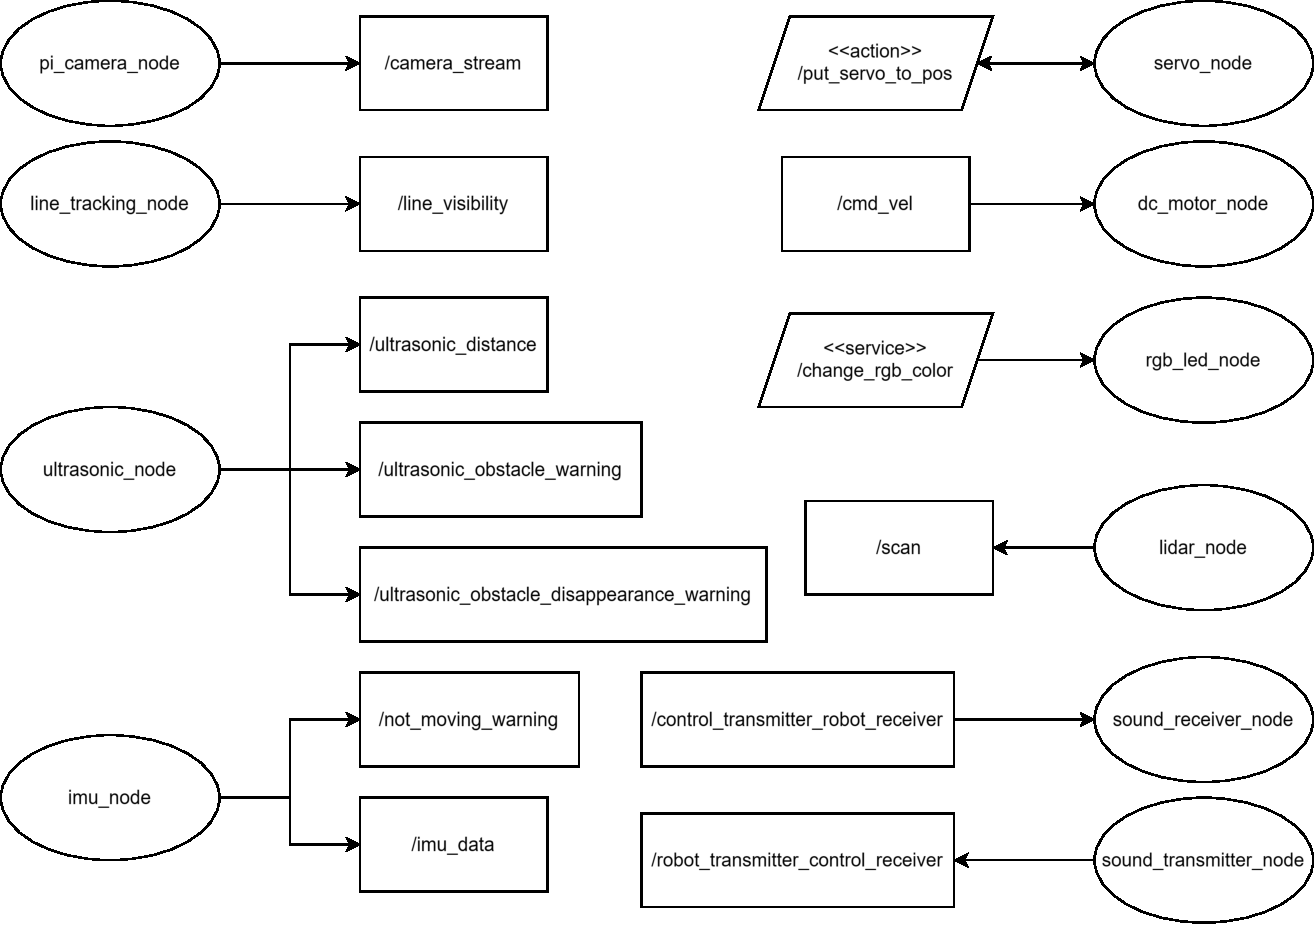
\includegraphics[scale=0.5]{obrazky-figures/hardware_nodes.pdf}
	\caption{}
	\label{}
\end{figure}

\subsection*{Komponenty součástí adeept kitu}
Základem robota je stavebnice adeept s základními komponentami.

\subsubsection*{Motory}
Jak už bylo řečeno v teoretické části, na Robot HAT nachází full-bridge ovladač. Řídící uzel \verb|dc_motor_node| s tímto obvodem interaguje přímo pomocí GPIO pinů. K ovládání GPIO pinů byl použit Python modul \verb|RPi.GPIO|. Zbytek řízení motorů už realizuje přímo uzel nastavování hodnot vývodů \verb|In| a úpravou PWM frekvence na vývodu \verb|En|.

Od zbytku ROS2 systému pak uzel přijímá příkazy pomocí \verb|cmd_vel|(command velocity) topicu. Jedná se o běžně používané jméno pro zasílání příkazů na pohyb robota. Zprávy v tomto topicu jsou typu \verb|geometry_msgs/msg/Twist|. Robot s diferenciální nápravou se může pohybovat pouze v přímo vpřed / vzad, nebo otáčet do stran. Z Twist zprávy jsou pro něj tedy důležité pouze dvě složky \verb|linear.x| a \verb|angular.z|. Pomocí nich lze spočítat výsledná rychlost otáčení kol na jedné a druhé straně.

$$\omega_L = \frac{V - \omega * b/2}{r}$$
$$\omega_R = \frac{V + \omega * b/2}{r}$$

\noindent Kde $\omega_L$ a $\omega_R$ jsou výsledné rychlosti motorů v $[rad/s]$. $V$ je zadaná lineární a $\omega$ angulární rychlost v $[m/s] a [rad/s]$. $b$ je rozpětí mezi koly a $r$ poloměr kola v $[m]$. \cite{diff_drive}

\begin{figure}[h!]
	\centering
	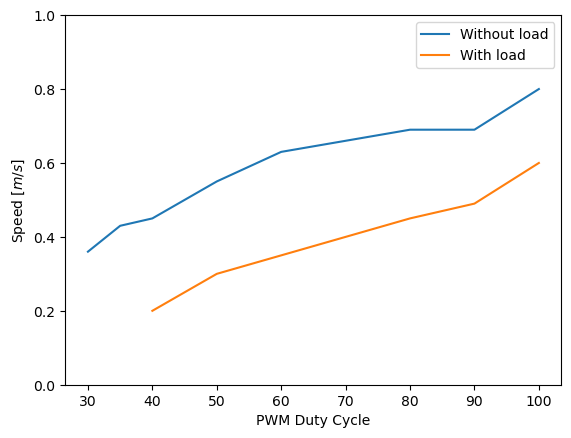
\includegraphics[scale=0.75]{obrazky-figures/motors_graph.png}
	\caption{}
	\label{}
\end{figure}
Tento graf zobrazuje rychlosti robota s různými hodnotami PWM střídy. Měření pod zátěží bylo zaznamenáno jako ujetá vzdálenost za jednu vteřinu. Bez zátěže byl změřen čas jedné otáčky a ten následně přepočítán na vzdálenost. Je zde vidět, že hodnoty střídy menší, než 30-40\% nedokážou překonat fyzikální jevy(setrvačnost, tření, \dots) aby motory vůbec roztočily. Zároveň růst není zcela lineární, ale hodnoty jsou dostatečně blízko aby je řídící uzel lineárnost předpokládal.

Problém s motory, který se pořádně projevil až u jednoho z rozšíření je jízda po oblouku (současný pohyb vpřed a zatáčení). Nejsem si zcela jistý co je příčinou tohoto jevu, ale hodnoty vypočítané využitím předchozího vzorce nevedou na předpokládaný oblouk. K ujištění, že není chyba na mé straně, byl v pozdější fázi využit framework ros2\_control k řízení motorů. Ten realizuje výpočet kinematiky vlastním vestavěným ovladačem a výsledek byl stejný. Zde je důležité zmínit, že robot se po oblouku pohybovat dokáže, pouze na to vyžaduje větší rozdíl mezi rychlostmi kol. Předpokládanou příčinou je použití levných motorů, protože pokud je na jeden z nich vyvinuta větší váha často se přestane otáčet a naopak když ostatní motory jedou vyšší rychlostí můžou být ty na druhé straně \uv{taženy} za nimi i přes to že by se měly otáčet pomaleji.

\subsubsection*{Servo}
Adeept AWD 4WD je vybaven pouze jedním servem, které slouží k ovládání úhlu natočení kamery. Konkrétní použitý model je Adeept AD002. Úhel serva se nastavuje pomocí PWM signálu. Jeho generování zajišťuje čip PCA9685, který je součástí Robot HAT. V softwaru je k jeho řízení využita knihovna \verb|Adafruit_PCA9685|. Řídící uzel serva se jmenuje \verb|servo_node| a z pohledu ROS2 systému se jedná o demonstraci jednoduchého action serveru. Server příjme požadavek a zkontroluje limity. 
Rozsah pohybu serva je větší než prostor pro kameru, řídící uzel proto omezuje maximální a minimální hodnoty natočení serva. Následně pomalu otáčí servem a v průběhu odesílá feedback zprávy s aktuálním úhlem.

\subsubsection*{Kamera}
Zachytávání snímků kamery je realizováno pomocí knihovny OpenCV. Aby bylo možno dosáhnout relativně krátké odezvy při přehrávání videa není obraz zaznamenáván v nativním rozlišení a snímkovací frekvenci kamery, ale byly použity snížené hodnoty. V základním konfiguraci je použito rozlišení 960 na 540 pixelů a snímkovací frekvence 20hz.
Pro přenos snímků v ROS2 systému je použita zpráva vestavěného typu \verb|CompressedImage|. Před odesláním jsou ještě data zakódována do \verb|jpeg| formátu pomocí funkce z \verb|OpenCV| knihovny.

\begin{center}
	\begin{tabular}{| l | c c c |}
		\hline
		Formát & Base64 & Image & CompressedImage \\ 
		\hline
		Velikost zprávy: & 0,24 MB & 1,56 MB & 0,17 MB  \\ 
		\hline 
	\end{tabular} \\ \vspace*{0.5em}
	Hodnoty v této tabulce pocházejí z utility \verb|$ros2 topic bw|
\end{center}

Před finálním rozhodnutím o použití \verb|CompressedImage| formátu bylo experimentováno také se zprávami typu \verb|Image|. Tento typ obsahuje více rozšiřujících informací o přenášeném obrázku jako jeho rozměry, použité kódování a podobně. Na první pohled se tedy zdá jako vhodnější formát. Snímky kamery jsou ale přenášené mezi dvěma různými zařízeními pomocí wifi připojení. Tento objemově větší formát tak přináší příliš velké zpoždění, které překonává použitelné hranice pro streamování. Na počátku vývoje byl použit ještě třetí možný přístup. Ten však nevyužívá ROS2 funkcionality a proto byl později změněn. Tímto přístupem je zakódování přenášených snímků do \verb|base64| formátu a následné přenesení jako jednoduchou \verb|string| zprávu. Base64 kódování se ukázalo jako zcela funkční možnost a dokonce dosahuje podobných výsledků ve zpoždění jako má \verb|CompressedImage|.
 
\subsubsection*{Ultrazvukový senzor}
Jedná o model hc-sr04. Ten dokáže měřit vzdálenost od 2cm do 400cm s přesností na 3mm. Získávání dat z ultrazvukového senzoru je relativně jednoduché a nevyžaduje tedy externí knihovnu. Interakce se senzorem je zajištěna pomocí GPIO pinů. K jejich ovládání je opět použit modul \verb|RPi.GPIO|. 

Uzel zahajuje komunikaci vysláním pulzu na trig vodiči. V ten moment začne senzor měřit a uzel jen čeká na odpověď. Ta přijde na echo pinu. Začíná tím, ze senzor nastaví echo pin na hodnotu jedna. V ten moment si uzel uloží časovou značku. Poté počká, než se echo pin vrátí zpět do nuly. V ten moment získává druhou značku. Pomocí těchto dvou momentů lze vypočítat výslednou vzdálenost. Výpočet vzdálenosti je podrobněji popsán v teoretické části (str: \pageref{theory:ultrasonic}).

Do ROS2 systému tento uzel odesílá kromě pravidelné informace o aktuální vzdálenosti také dvě další zprávy. Tou první je jednoduché varování o detekci překážky. Uzel varuje pokud je naměřená vzdálenost menší než zadaná hranice. Toto varování však zaznamená pouze překážky přímo před robotem. Druhá zpráva tak doplňuje tu první. Snaží se detekovat překážky, které můžou stále vést ke kolizi, ale senzor je již nedetekuje. 

\begin{figure}[h!]
	\centering
	\begin{minipage}[c]{0.5\textwidth}
		\centering
		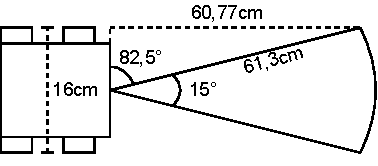
\includegraphics[scale=1.0]{obrazky-figures/ultrasonic_blind_spot.pdf}
	\end{minipage}%
	\begin{minipage}[c]{0.5\textwidth}
			$$\cos(82.5^\circ) = \frac{8\text{cm}}{\text{prepona}} \Rightarrow 61.3\text{cm}$$
			$$\sin(82.5^\circ) = \frac{\text{protilehla}}{61.3\text{cm}} \Rightarrow 60.77\text{cm}$$
	\end{minipage}
	\caption{}
	\label{}
\end{figure}

Tento obrázek demonstruje případy, které se snaží druhé varování zachytit. Je na něm vidět, že existuje meziprostor, ve kterém může překážka zmizet ze senzoru, ale i přes to vést ke kolizi s robotem. Tento meziprostor je na jedné straně ohraničen vzdáleností pro klasické detekování překážek, například 20cm. Na druhé straně lze hranici vypočítat pomocí úhlu ve kterém senzor detekuje překážky a šířky robota.
V tomto případě se jedná o 61cm. Druhá zpráva tedy informuje o tom, že nějaká překážka zmizela z radaru v této potenciálně nebezpečné zóně.

\subsubsection*{Sledování čáry}
Posledním praktickým senzorem kterým robot Adeept AWR disponuje je třícestný senzor na sledování čáry.
Komunikace je v tomto případě ještě jednodušší. Senzor má tři výstupy připojené na tři GPIO piny. Každá dvojice vysílače a senzoru má svůj vlastní vývod. Hodnoty těchto výstupů obsahují aktuální stav detekování čáry. Z pohledu uzlu tak stačí pravidelně číst hodnoty a odesílat je dále do ROS2 systému. Opět k tomuto účelu využívá modul \verb|RPi.GPIO|.

\subsubsection*{Led}
Součástí Adeept sady je také několik adresovatelných led diod. Jedná se o hardware, který je pro hlavní funkcionalitu naprosto nepotřebný. Ponechat však na robotu nevyužitý a neovládatelný hardware nedává smysl. Proto byl nakonec implementován uzel na jejich řízení. Z pohledu ROS2 se jedná o klasický service server. Požadavky obsahují RGB barevnou hodnotu, pro nastavení všech led zároveň. Řízení tohoto typu led pásku je komplexnější záležitost a proto je k jeho ovládání využit python modul \verb|rpi_ws281x|. 
Aby tento modul mohl správně pracovat, vyžaduje spuštění s vyššími oprávněními. Důvodem k tomuto požadavku je fakt, že vnitřně využívá kód v jazyce C, který pracuje s GPIO piny přímo přes /dev/mem. Problém nastává v tom, že ROS2 při svém běhu nevyžaduje a tedy ani nepoužívá zvýšená oprávnění. Z toho důvodu na tyto případy není připravený a prosté přidání \verb|sudo| před spouštěcí příkaz nefunguje. Toto lze obejít a spustit uzel s oprávněními podobnými příkazu \verb|sudo|. Avšak uzly spuštěné tímto způsobem nedokážou komunikovat s klasicky spuštěnými uzly. 
Problém je ve výsledku vyřešen použitím druhého skriptu. Ten obsahuje jen minimum kódu pro ovládání zmíněného modulu. V \verb|sudoers| je tomuto konkrétnímu souboru umožněno spuštění se \verb|sudo| oprávněními, aniž by bylo vyžadováno heslo. Tento skript je následně volán z hlavního uzlu použitím \verb|subprocess| modulu. Jedná se o velmi neelegantní řešení. A vzhledem k tomu, že se svícení LED diodami není důležitá funkcionalita a zbytečně upravuje systémově důležitý soubor \verb|sudoers| je tento krok v instalačním skriptu separátně volitelný.

\subsection*{Další hardware nad rámec Adeept Kitu}
V tento moment byly probrány všechny uzly které řídí komponenty původní stavebnice Adeept Awr 4WD. Následuje popis rozšíření původního hardwaru o další komponenty, které buď rozšiřují funkcionalitu robota, nebo usnadňují jeho použití.

\subsubsection*{Nabíjení}
V originální konfiguraci napájí robota dvě sériově zapojené 18650 baterie. V tomto zapojení poskytují napětí 8V s maximálním proudem 4A. Součástí Adeept Kitu jsou kolébky na baterie. Ty jsou pak přímo připojené k zátěži(robot HAT). Nabíjení baterií pak musí být realizováno externě. Tento způsob je nepohodlný hlavně proto, že přístup ke kolébkám vyžaduje sundání kol robota. Prvním rozšířením je tedy přidání BMS a nabíjecí desky. 
Nejrozšířenějším způsobem nabíjení baterií 18650 jsou desky s čipem TP4056. Jedná se o hojně dostupný produkt, který lze koupit v různých kombinacích ochran a vstupů pro napájení. Problémem je fakt, že tyto desky jsou určeny pro nabíjení jedné 18650 baterie. Potenciálním řešením pro paralelní zapojení je použití více těchto desek. Pro baterie zapojené sériově, které používá tento robot, jsou tyto desky nevhodné.
Lepší přístup je využití Battery Management System. Jak z názvu vyplývá, jedná se o desku pro správu baterií. BMS se vyrábí specificky pro konkrétní zapojení, které bude monitorovat. Použitý model je typu 2S, pro dvě sériově zapojené baterie. Kromě kladného a záporného pólu disponuje také připojením pro bod mezi bateriemi. Tento bod umožňuje desce monitorovat stav každé z baterií zvlášť.
V kombinaci s BMS je dále využita samotná nabíjecí deska. Jedná se o model, který na rozdíl od TP4056 nabíjí dvakrát vyšším nabíjecím napětím.

\begin{figure}[h!]
	\centering
	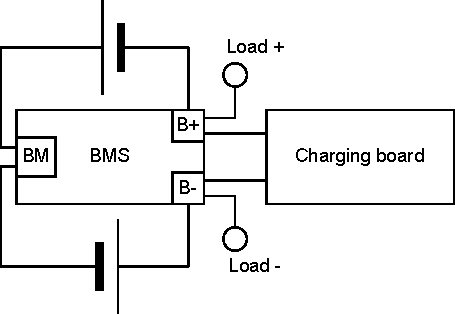
\includegraphics[scale=0.75]{obrazky-figures/battery_circuite.pdf}
	\caption{Zapojení BMS a nabíjecí desky}
	\label{}
\end{figure}

\subsubsection*{Inertial Mesurement Unit - IMU}
Druhým rozšířením oproti originální stavebnici je přidání IMU senzoru. Konkrétně se jedná o model MPU5060. Ten disponuje tříosým akcelerometrem a gyroskopem. Uzel na jeho ovládání, využívá knihovnu třetí strany \verb|mpu6050-raspberrypi|. Získaná data je nejprve potřeba vyčistit. Přímo v hardwaru je implementována dolní propusť, sloužící k eliminaci vibrací a jiných nechtěných vlivů. Nastavuje se zápisem do konfiguračního registru na adrese \verb|0x1A|, což lze provést využitím knihovní funkce \verb|set_filter_range|. Získaná data se nadále čistí softwarově. Protože se jedná o levný senzor, tak není zcela přesný a čtené hodnoty obsahují malé odchylky i v době, kdy by měly být nula. Proto se v softwaru aplikuje offset, který posune výsledky blíže k reálným hodnotám. Dalším krokem může být získaná data průměrovat mezi více vzorky a dosáhnout tak ještě většího utlumení výkyvů. 

Do ROS2 systému tento uzel nejprve odesílá aktuální hodnoty senzoru a to pomocí zpráv typu Twist. Následně také posílá varování o kolizi, to detekuje v momentě, kdy \verb|cmd_vel| topic obsahuje příkaz pohybu, ale imu senzor čte výrazně odlišná data. Jako poslední tento uzel ještě odesílá odometrii. Odometrie udává transformaci aktuální pozice robota vůči počátku. Uzel tedy pravidelně čte hodnoty senzoru a integruje je, aby získal absolutní pozici robota. Největším problémem u získávání odometrie byl vliv gravitace na akcelerometr a fakt, že stejné zrychlení a zpomalení se né vždy rovná. Gravitace vede na špatné hodnoty zrychlení v případě, že je robot nakloněn v nebo proti směru pohybu. Různé hodnoty akcelerace a decelerace je pravděpodobně způsobená rychlou změnou, kterou senzor nestihne vzorkovat dostatečně rychle.

\begin{figure}[h!]
	\centering
	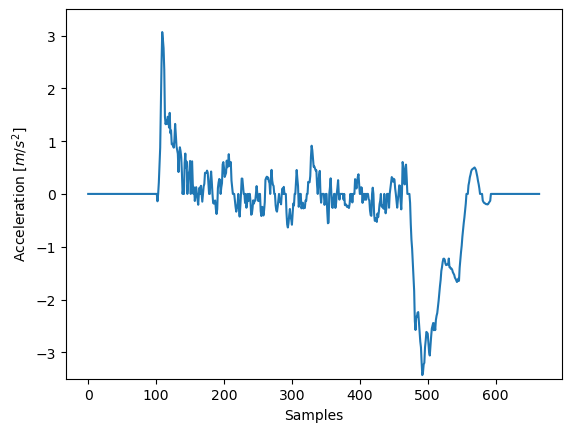
\includegraphics[scale=0.75]{obrazky-figures/accelerometer_graph.png}
	\caption{Výsledná rychlost po zintegrování tohoto grafu je -0.1496m/s}
	\label{}
\end{figure}
Tento graf zobrazuje případ kdy došlo k špatnému zaznamenání zpomalení a výsledná rychlost je následně záporná. Důležité je zmínit že případy kdy dochází k špatnému měření nejsou časté (cca každé 10). Z grafu je také vidět, že když se robot pohybuje je měření ovlivněno vibracemi motorů. Při testování se tento jev neprojevil dostatečně aby ovlivnil funkcionalitu.

Ve finální verzi jsou tyto vlivy převážně eliminovány využitím dat z \verb|cmd_vel| topicu. Tento přistup umožňuje ignorovat výkyvy dat získaných z imu senzoru v momentech, kdy by podle příkazů z \verb|cmd_vel| měl být robot statický.

\subsubsection*{Light Detection And Ranging - Lidar}
Posledním a zároveň nejkomplexnějším přidaným senzorem je lidar. Konkrétním použitým modelem je \verb|LD 19 D 300|. K jeho ovládání je využit již existující ROS2 balík \verb|ld19_lidar|. Výstupem tohoto uzlu jsou zprávy typu \verb|LaserScan| na topicu \verb|/scan|. Pro zajištění lepší kompatibility s \verb|slam_toolbox| byly v tomto uzlu provedeny menší změny v hlavičce odesílaných zpráv a byly odebrány nepotřebné výpisy, které zpomalovaly odesílání.

\subsubsection*{Přenos zvuku}
V zadání práce je zmíněno také téma teleprezence. Již probrané komponenty zajistí záznam videa a pohyb robota. K plnohodnotnější teleprezenci je však potřeba zajistit také přenos zvuku. A na rozdíl od videa ideálně obousměrně. Mozkem robota je mikropočítač Raspberry Pi 4, na kterém běží plnohodnotný operační systém. Připojení externích periferií jako mikrofon a reproduktory proto není problém. Řízení komponentů v tomto případě zajistí operační systém. ROS2 uzly se díky tomu můžou zaobírat pouze záznamem, přenosem a přehráváním dat. Pro tento účel byly vytvořeny dva uzly.

První slouží k nahrávání a odesílání audio dat. Pro záznam zvukového toku v reálném čase je použit Python modul \verb|sounddevice|. Tato knihovna kromě jiného disponuje také \verb|Stream| třídami. \verb|InputStream| umožňuje kontinuální záznam zvuku. Při inicializaci se jí(kromě dalších parametrů) předá callback funkce. Ta je volána vždy, když je potřeba zpracovat nasnímaný blok dat. ROS2 nedisponuje standardním typem zprávy pro přenos zvukových dat. Je zde využit vlastní typ složený ze dvou polí o prvcích typu \verb|float32|(každé pro jeden kanál).

Druhý uzel pak realizuje příjem a přehrávání získaných dat. Jedná se o obrácenou verzi předchozího uzlu. Přijímaná data jsou před přehráváním ukládána do bufferu. Důvodem je fakt, že přenos mezi dvěma uzly není zcela spolehlivý a datové bloky se mohou zpozdit. Pro přehrávání získaných dat je využita \verb|OutputStream| třída.

\begin{figure}[h!]
	\centering
	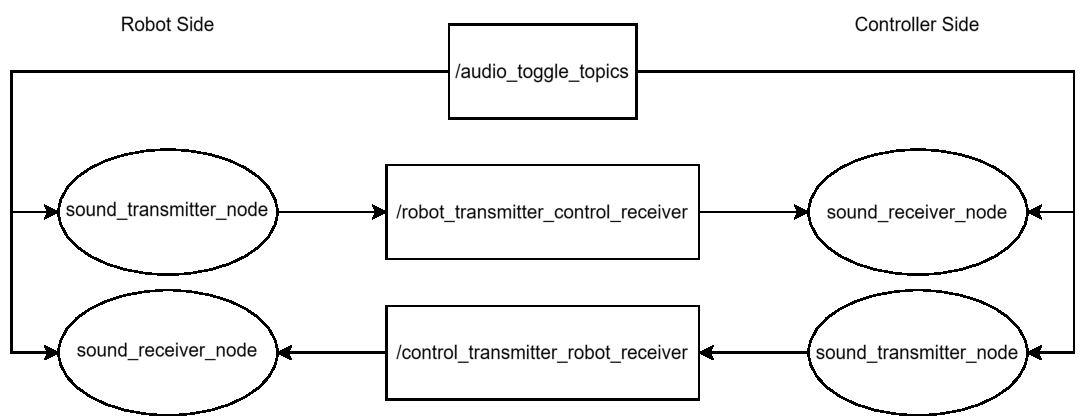
\includegraphics[scale=0.75]{obrazky-figures/audio_transfer_diagram.pdf}
	\caption{}
	\label{}
\end{figure}

Pro obousměrný přenos dat mezi robotem a stacionárním zařízením jsou použity dvě dvojice těchto uzlů. Oba uzly disponují mechanizmem pro pozastavení záznamu / přehrávání. 

\section{Řízení robota na vyšší úrovni}
V tento moment jsou implementovány všechny uzly pro ovládání komponent. Následuje sekce zabývající se řídícími uzly. Ty se nachází v balíku \verb|controllers|. Jejich úkolem je zpracovávat data z několika hardwarových uzlů současně a v podle získaných dat řídit robota jako celek.

\begin{figure}[h!]
	\centering
	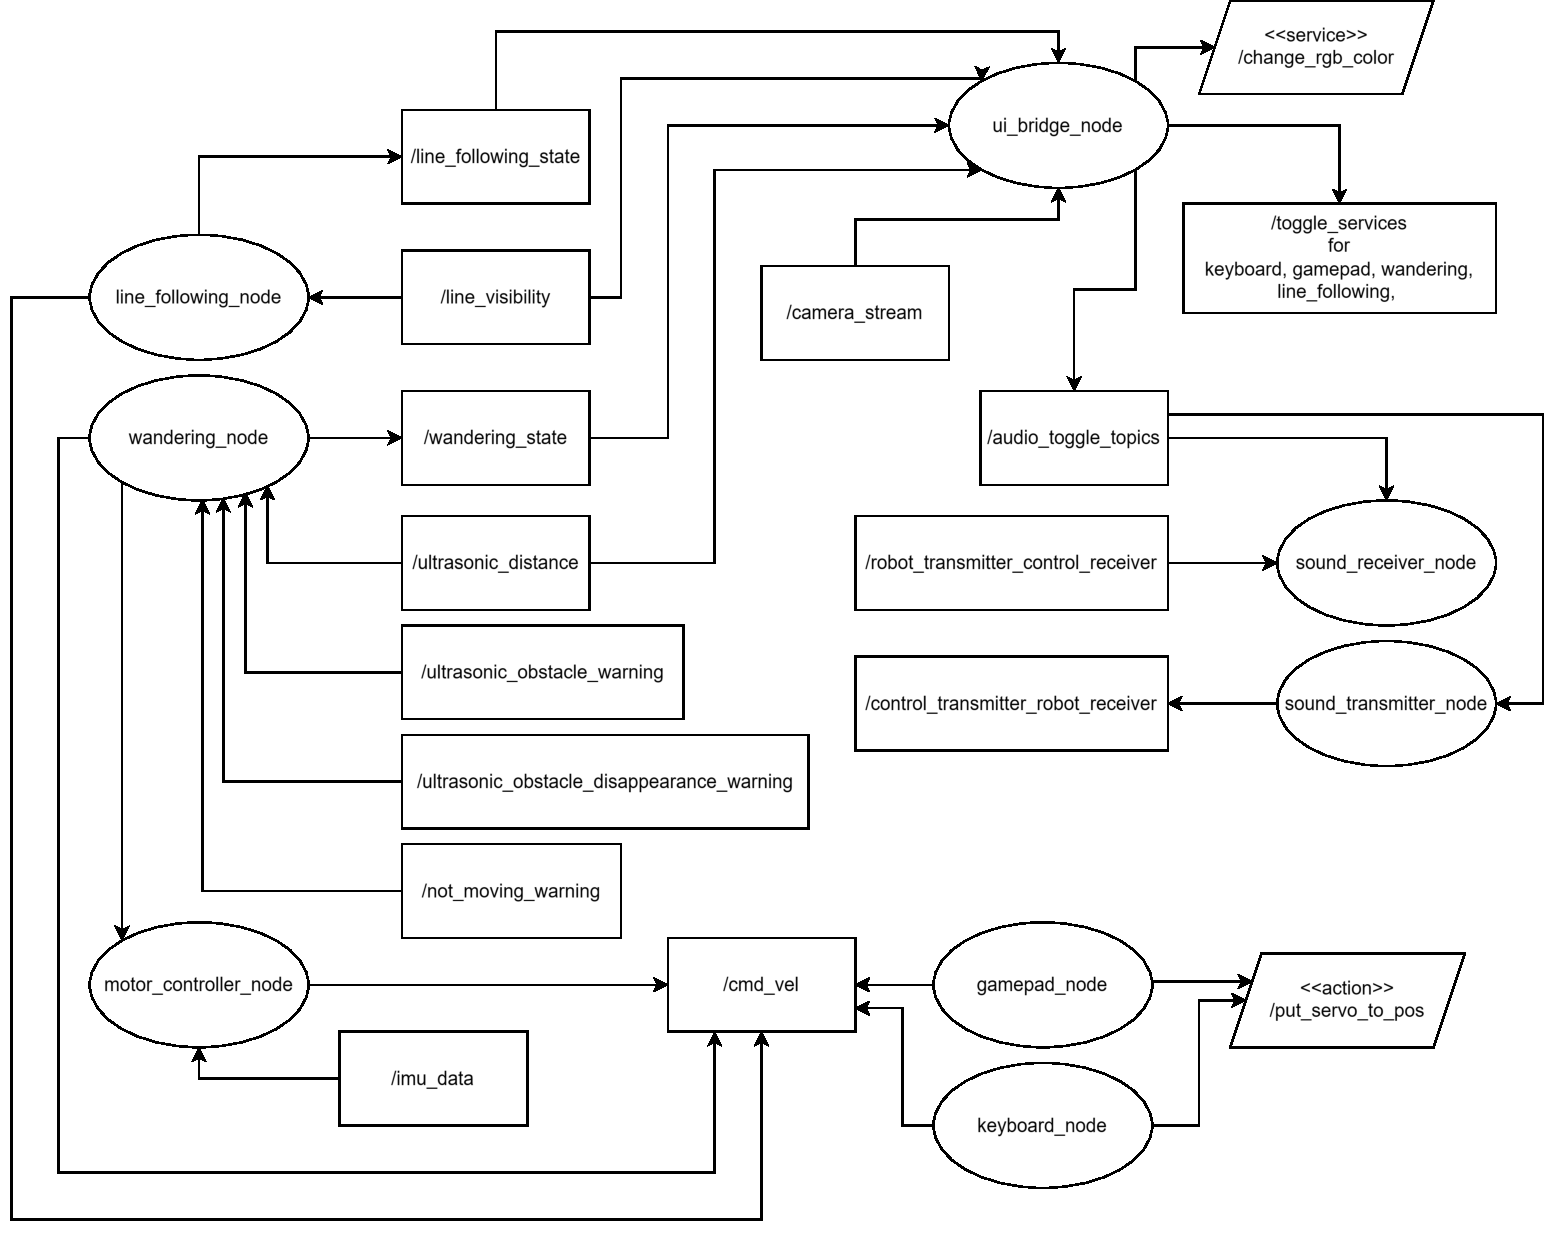
\includegraphics[scale=0.5]{obrazky-figures/controller_nodes.pdf}
	\caption{RQT Graph struktura řídícího systému}
	\label{}
\end{figure}

\subsubsection{Distribuovanost}
Řídící jednotky robotů bývají z pohledu výpočetního výkonu relativně slabá zařízení. Výpočetně náročné uzly mohou mýt problémy s během na těchto zařízeních. Z toho, a dalších důvodů umožňuje ROS2 distribuovat uzly mezi více fyzických zařízení. Z vývojářského pohledu je distribuovanost zcela v režii ROS2. Jediný předpoklad pro její fungování je vzájemná dosažitelnost zařízení přes počítačovou síť. Druhým požadavkem je nastavení stejného DOMAIN\_ID na obě zařízení, což je ve výchozím nastavení splněno. Ve správně fungujícím distribuovaném systému mohou uzly běžící na různých zařízeních navzájem komunikovat a interagovat stejně jako by běžely na jednom. V této práci se tedy předpokládá, že následující uzly poběží na druhém stacionárním zařízení. 

\subsection*{Manuální řízení}
Pro manuální řízení je systém vybaven dvěma uzly. První čte vstupy z klávesnice. Využívá k tomu modul \verb|pynput|. Druhý pak s pomocí \verb|pygame| knihovny získává vstupy ovladače. Oba uzly ovládají motory a servo pomocí jejich specifických rozhraní. Na obou uzlech se také nachází service servery pro příjem příkazů sloužících k zastavení nebo spuštění smyček, které zajišťují zachytávání vstupu od uživatele.

\begin{figure}[h!]
	\centering
	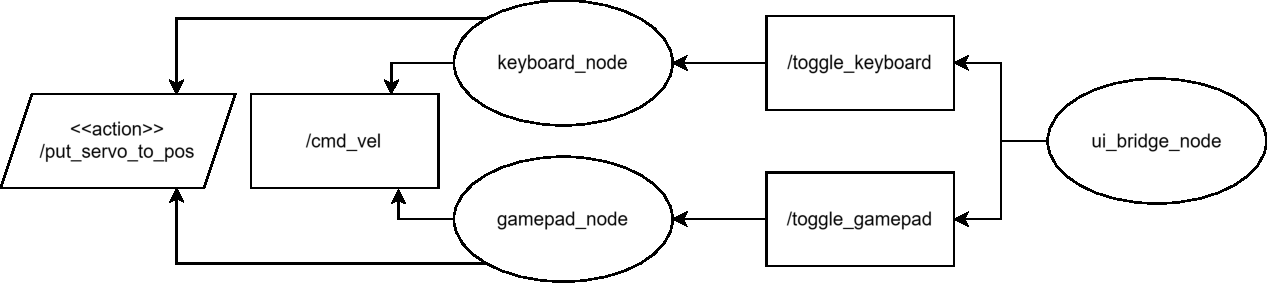
\includegraphics[scale=0.75]{obrazky-figures/manual_control_diagram.pdf}
	\caption{}
	\label{}
\end{figure}

\subsection*{Pomocný uzel pro přesné otáčení robota}
Vzhledem k tomu že použité motory nejsou opatřeny enkodéry, bez využití dalších senzorů, je jakékoli otáčení velice nepřesné. Motorům lze samozřejmě zadat konkrétní rychlost na určitý časový interval a dostat se tak na přibližně správnou orientaci. Ale opravdu se jedná jen o přibližný úhel z důvodů externích vlivů a nepřesností. Například setrvačnost hraje velkou roli při otáčení o úhly menší než 90° nebo při vyšším využití prostředků mikrokontroléru, můžou být reakce na příkazy zpožděné.
Proto byl vytvořen tento uzel, který využívá gyroskopická data z imu senzoru, aby zajistil, že se robot dokáže v případě potřeby otáčet o přesně dané úhly. V ROS2 systému se jedná o action server. Přijímá požadavky a následně zasílá příkazy na \verb|cmd\_vel| topic. Podle hodnot získaných z imu pak postupně snižuje rychlost otáčení v závislosti na vzdálenosti od cílového úhlu. 

\begin{figure}[h!]
	\centering
	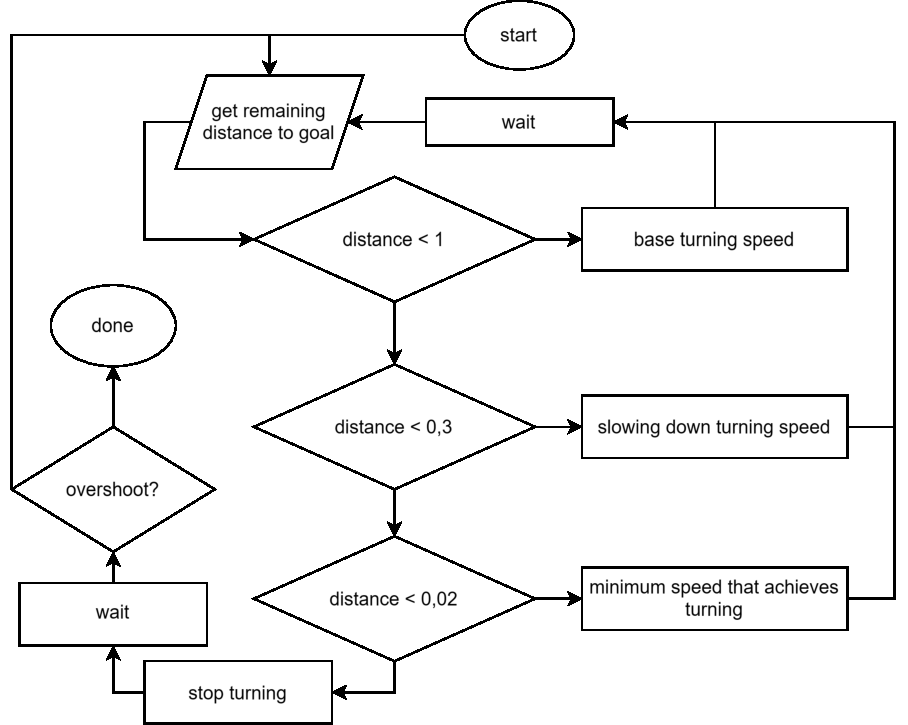
\includegraphics[scale=0.75]{obrazky-figures/precise_turning.pdf}
	\caption{}
	\label{}
\end{figure}

Z pohledu demonstrace ROS2 funkcionality tento uzel využívá pokročilejší možnosti action serveru. Konkrétně se jedná o schopnost definování a předání vlastních callback funkcí, pro jednotlivé události související s akcemi. V případě standardního použití action serveru se pracuje pouze s execute callback funkcí. V jejím těle by mělo proběhnou celé zpracování požadavku.

V případě tohoto uzlu tento přístup nelze použít. Každý spuštěný ROS2 uzel má svůj vlastní execution loop, funkce spin(). Když se uzel točí, reaguje na události a volá callback funkce. V průběhu vykonávání takové funkce se však uzel netočí. A zde nastává problém. V průběhu vykonávání execute callbacku by tento uzel potřebovat průběžná data z imu senzoru. Ty se však získávají v subscriber callback funkci, která se nezavolá v průběhu vykonávání execute callbacku. Proto bylo potřeba použít další callback funkce action serveru k zprovoznění tohoto uzlu. 
 
\begin{itemize}
	\item{goal\_callback}
	\begin{itemize}
		\item{vyvolá se při příchodu požadavku, rozhoduje o jeho přijmutí nebo zamítnutí}
		\item{pokud probíhá vykonávání požadavku jsou nově příchozí zamítnuty, důvodem je fakt, že po dokončení aktuání obsluhy bude orientace robota jiná, než když byly požadavky zaslány a tudíž s největší praděpodobností již nebudou platné}
	\end{itemize}
	\item{handle\_accepted\_callback}
	\begin{itemize}
		\item{vyvolá se po přijmutí cíle}
		\item{v tomto uzlu zahajuje zpracování požadavku}
	\end{itemize}
	\item{execute\_callback}
	\begin{itemize}
		\item{měl by obsahovat hlavní funkcionalitu action serveru, rozhoduje o úspěchu požadavku}
		\item{v tomto uzlu je volán aby ukončil vykonávání požadavku}
	\end{itemize}
	\item{cancel\_callback}
	\begin{itemize}
		\item{vyvolán pří přijmutí požadavku na zrušení akce od klienta, rozhoduje o přijmutí tohoto požadavku}
	\end{itemize}
\end{itemize} 

\begin{algorithm}[h!]
	\label{}
	\caption{\textsc{Action Server Callbacks}}
	
	\DontPrintSemicolon
	\SetAlgoNoLine
	\SetAlgoNlRelativeSize{-1}
	\SetNlSty{}{}{:}
	\SetNlSkip{-1.1em}
	
	\BlankLine \Indp\Indpp
	
	\texttt{def goal\_callback(self, goal\_request):}\;
	\Indp\Indp
	\texttt{if self.goal\_handle is not None and self.goal\_handle.is\_active:}\;
	\Indp\Indp
	\texttt{return GoalResponse.REJECT}\;
	\Indm\Indm
	\texttt{else:}\;
	\Indp\Indp
	\texttt{return GoalResponse.ACCEPT}\;

\end{algorithm}

\subsection*{Bloudění}
Náhodné bloudění robota po místnosti je základním autonomním pohybem. Cílem tohoto režimu je náhodný pohyb robota v prostoru, s cílem vyhýbat se překážkám.

K získávání informací o svém okolí používá tento uzel data ze dvou senzorů. Prvním je ultrazvukový senzor vzdálenosti. Ten je umístěn na přední straně robota a detekuje překážky v 15° úhlu před robotem. Druhým použitým senzorem je IMU. Přímo z něj získává pouze varování o kolizi. Nepřímo jej využívá při přesném otáčení s využitím  \verb|motor_controller_node| uzlu.

\begin{figure}[h!]
	\centering
	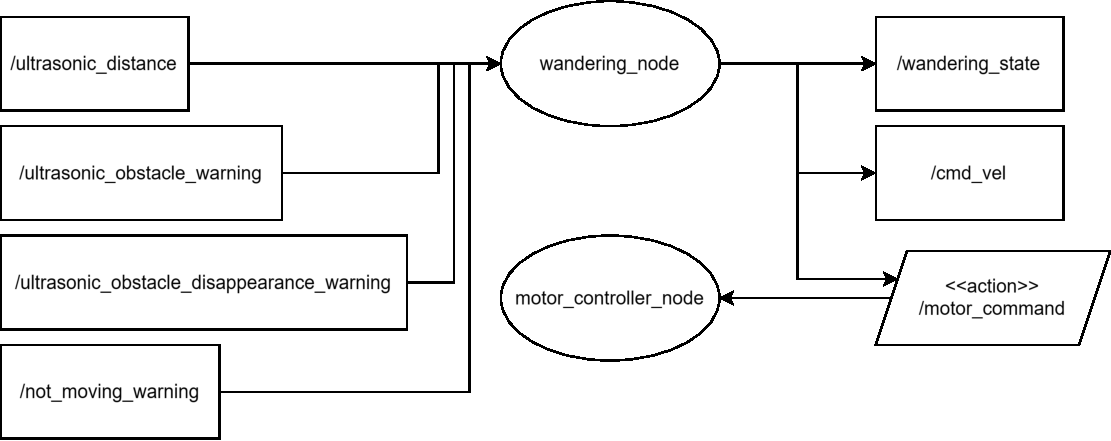
\includegraphics[scale=0.75]{obrazky-figures/wandering_rqt.pdf}
	\caption{}
	\label{}
\end{figure}

Jádrem implementace je konečný automat. Ten byl v průběhu vývoje obohacen o další funkcionalitu. Primárně bylo potřeba reagovat na externí události a volat funkce jiných uzlů. Výsledný kód tedy není čistým konečným automatem. Z abstraktnějšího pohledu tento režim provádí tři hlavní akce. Tou první je jednoduchý pohyb vpřed. Další dvě zajímavější akce pak realizují vyhýbání překážkám. Úvodními stavy těchto akcí je \verb|OBSTACLE| a \verb|SCAN_START|.

\verb|OBSTACLE| má za úkol reagovat a vyřešit překážky nacházející se přímo před robotem. Detekování a přechod do tohoto stavu zajišťuje buď zpráva od ultrazvukového senzoru o překážce nacházející se příliš blízko, nebo zpráva od imu senzoru varující o tom, že \verb|cmd_vel| vyslala příkaz o pohybu vpřed avšak akcelerometr změnu nezaznamenal, což implikuje, že se robot opírá o nějakou překážku.

Algoritmus nalezení volné cesty demonstruje následující diagram. Ve zkratce funguje následovně. V náhodném pořadí zkontroluje obě strany robota. Pokud na jedné z nich najde volný prostor ihned tudy pokračuje v jízdě. Pokud je v obou směrech překážka, vrací se zpět odkud přijel.

\begin{figure}[h!]
	\centering
	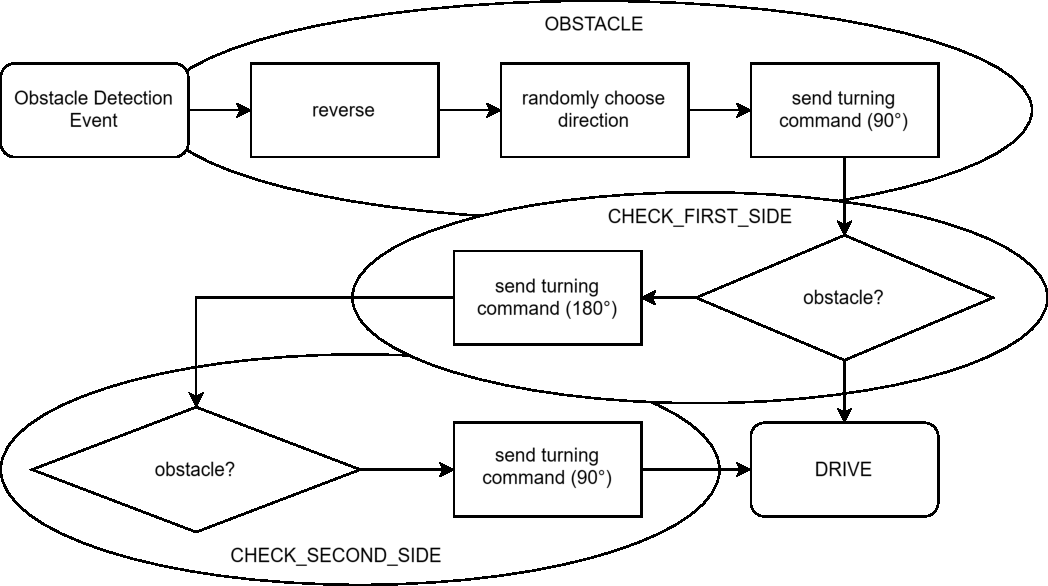
\includegraphics[scale=0.75]{obrazky-figures/wandering_obstacle_diagram.pdf}
	\caption{Algoritmus vyhnutí se překážky přímo před robotem.}
	\label{}
\end{figure}

\verb|SCAN_START| je oproti předchozímu chování více obezřetné. Jeho originálním záměrem bylo hledat překážky, které zmizely z ultrazvukového senzoru (více o tomto jevu v kapitole x). Tato funkcionalita byla následně rozšířena a ve finální verzi probíhá pravidelné skenování prostoru před robotem. Vzhledem k tomu, že se jedná o preventivní akci, nesnaží se vyhýbat překážkám přímo před robotem. Jeho cílem je nalézt překážky v blízkosti aktuální trajektorie robota. A v reakci na ně odklonit směr pohybu dále od nich. Pokud skenování nalezne překážku přímo před robotem, pokračuje v pohybu vpřed. Tím efektivně přenechává vyřešení tohoto problému \verb|OBSTACLE| stavu. Možné přechody do úvodního stavu skenování lze vyvodit z předchozího textu. Prvním je přijmutí varování o detekci zmizelé překážky od ultrazvukového senzoru. Druhým je pak pravidelné volání ze stavu \verb|DRIVE|. 

Algoritmu skenování je opět zobrazen na následujícím diagramu. Úhel hledání překážek je 90°. Celkem je provedeno šest čtení začínající na úhlu -45° a končící na +45°. Získaná data jsou následně interpretovány a je učiněna adekvátní reakce.

\begin{figure}[h!]
	\centering
	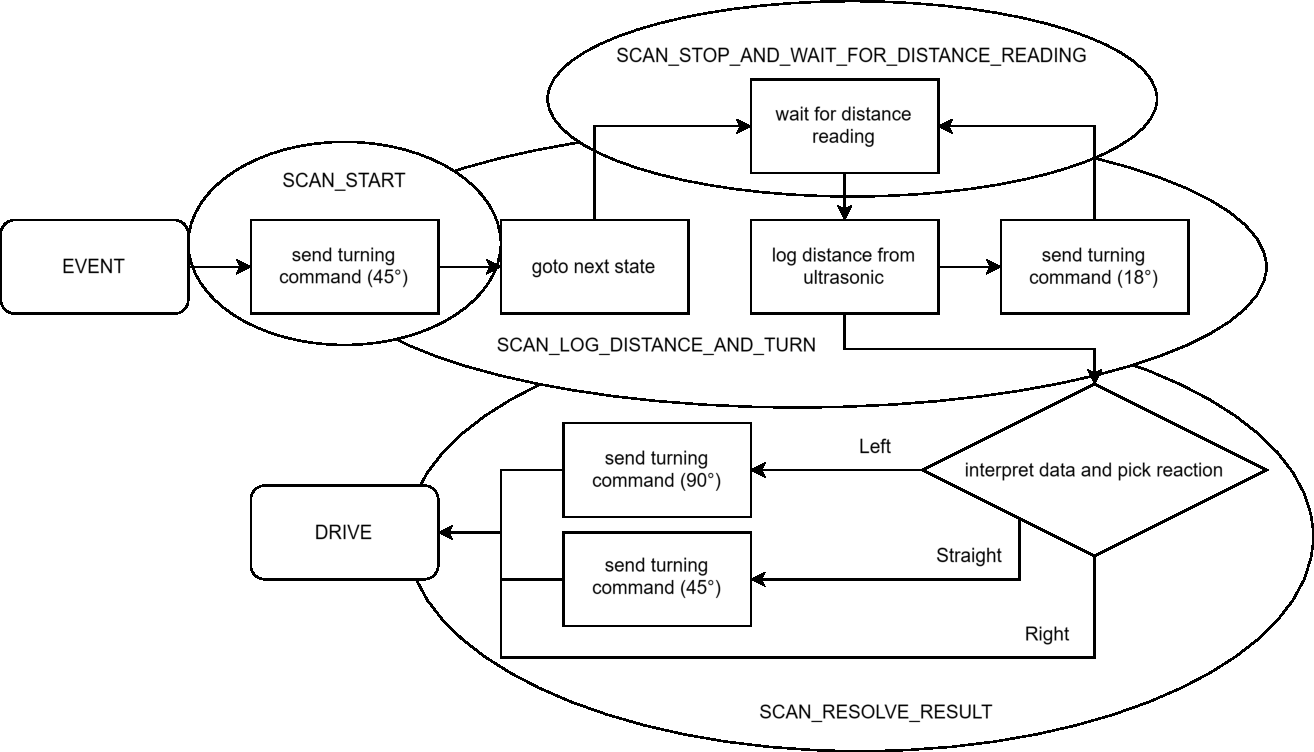
\includegraphics[scale=0.65]{obrazky-figures/wandering_scan_diagram.pdf}
	\caption{Algoritmus preventivního hledání překážek.}
	\label{}
\end{figure}

\subsection*{Sledování čáry}
Sledování čáry je v robotice známý úkol a na vyšších úrovních se v této disciplíně pořádají závody. Avšak v základním provedení se jedná o jednoduchý úkol. Tato funkcionalita je implementována hlavně z toho důvodu, že robot disponuje senzorem, který je k sledování čáry určený.

Implementace je proveden použitím konečného automatu. Použitý senzor je třícestný. Automat tedy bude obsahovat s $2^3$ stavů. Z tohoto počtu jsou dva stavy koncové a to 101, protože se jedná o nevalidní stav a 000 indikující ztrátu čáry. Mezi všemi ostatními lze navzájem přecházet. Následující stav se volí podle aktuálních hodnot senzorů. Přechodová logika byla následně obohacena o další podmínky s cílem reagovat na ztrátu čáry. To umožnilo následovat čáru s ostrými zatáčkami (pravý úhel a více). A také překonávat krátké přerušení v čáře. Zde je důležité zmínit, že tato funkcionalita byla testována hlavně v simulátoru a i tam má poměrně hodně nedostatků. 

\section{Spouštěcí Soubory (Launch files)}
Každý uzel ve výsledném systému má k sobě vytvořený spouštěcí soubor. Ve většině případů se jedná o jednoduché soubory jejichž úkolem je načtení a předání konfiguračního souboru spouštěnému uzlu. Některé parametry je vhodné změnit také při spouštění uzlu. Spouštěcí soubory, které toto umožňují, musí tento parametr explicitně definovat. 
\begin{verbatim}
	ros2 launch lauch.py param_name:=value
\end{verbatim}
Ve složce \verb|ros2_ws/launch| se nachází hromadné spouštěcí soubory. Ty mají za úkol využít nižších spouštěcích souborů k nastartování větší části systému zároveň. Díky této hierarchické struktuře už není potřeba řešit předávání všech parametrů a lze se zaměřit jen na to důležité. Pokud jsou volány soubory, které parametry explicitně definují, lze je v tento moment přepsat, stejně jako by to udělal uživatel z příkazové řádky. Příkladem využití této funkcionality je řídící uzel \verb|wandering_node|. Pokud je tento uzel spuštěn manuálně, předpokládá se, že v systému žádný jiný řídící uzel neběží. Může tedy zahájit vykonávání hned po inicializaci, aniž by jeho příkazy kolidovaly s dalšími řídícími uzly. V případě, že je však volán jako součást hromadného spouštění, přepíše se výchozí hodnota parametru \verb|start_right_away| a všechny řídící uzly tak budou po inicializaci čekat na další příkaz.
\begin{verbatim}
IncludeLaunchDescription(
    launch_goal,
    launch_arguments={'start_right_away': 'false'}.items()
)
\end{verbatim}

Hromadné spouštěcí soubory startují mnoho uzlů zároveň. Běžným požadavkem tak je výměna několika málo uzlů za jiné. V takovém případě by bylo potřeba vytvořit druhý, převážně totožný soubor. K eliminaci tohoto problému slouží podmíněné spouštění. Jeho jednoduchou verzi využívá \verb|adeept_robot_launch.py|. V tomto případě slouží k rozhodnutí, který ze dvou možných uzlů k řízení motorů bude použit. Cílům spouštěcího souboru se do proměnné \verb|condition| přidá podmínka. Jedná se o speciální třídy (\verb|Ifcondition|, \verb|Unlesscondition|, \dots). V konstruktoru se jim předává true / false výraz. Jeho hodnotu lze získat například z parametru. Podmíněné spouštění může být i komplexnější a to v kombinací s \verb|PythonExpression|. Tato třída je použita v \verb|gazebo_simulation_launch.py| souboru, kde se porovnáním hodnoty parametru určuje, který svět bude spuštěn.
\begin{verbatim}
IncludeLaunchDescription(
    launch_goal,
    condition=IfCondition(
        PythonExpression([
            '"', world_select_val, '"', ' == "wandering"'
        ])
    )
)
\end{verbatim}

Komplexnější spouštěcí soubory často potřebují větší kontrolu nad tím, kdy dojde ke provedení jednotlivých cílů. V případě, že je potřeba pouze opozdit provedení některého z cílů lze využít \verb|TimerAction|. Jedná se o třídu, která spustí daný cíl až po předem stanoveném časovém intervalu. Tato funkce je využita při spouštění \verb|ros2_control| v souboru \verb|diffdrive_launch.py|, kde slouží k zpoždění \uv{spawn} ovladače až po dokončení inicializace pluginu.
\begin{verbatim}
TimerAction(
    period=10.0,
    actions=[
        Node()
    ]
)
\end{verbatim}

K přesnějšímu řízení pak slouží event handlery. Ty umožňují přesnější kontrolu nad tím, kdy dojde k vykonání jednotlivých cílů. Typickými událostmi jsou spuštění a ukončení procesu, případně, pokud se jedná o lifecycle uzly, také reakce na přechody do konkrétních stavů. Obsluha událostí je využita přímo v balíku gazebo simulace v souboru \verb|gazebo_world_launch.py|. Je zde celý řetěz těchto obsluh, které postupně spustí simulaci, přeloží \verb|xacro| model na \verb|urdf|, \uv{spawnou} jej do simulace a po jejím ukončení ještě uklidí vygenerovaný \verb|urdf|.
\begin{verbatim}
RegisterEventHandler(
    OnProcessStart(
        target_action=simulator,
        on_start=convert_xacro
    )
)
\end{verbatim}

\section{Model Robota}
Model robota slouží k předání informace o jeho struktuře, vzhledu a fyzikálních vlastnostech dalším částem ROS2 systému. Formát pro definici modelu, který ROS2 používá je \verb|urdf|. Většina nástrojů však nepracuje přímo s definicí v \verb|urdf| formátu, ale získává tyto informace z \verb|/tf| subsystému. Zpracování, interpretaci a následné odesílání informací o aktuálním stavu robota zajišťuje \verb|robot_state_publisher|. Jedná se o oficiální ROS2 uzel. Vstupem tohoto uzlu je \verb|urdf| model robota. Prvním výstupem je odesílání statických i dynamických transformací do \verb|/tf| systému. Aby mohl odesílat dynamické tranformace musí mít informaci o aktuálních natočení kloubů. Ty získává posloucháním \verb|joint_states| topicu.

Druhým výstupem tohoto uzlu je topic \verb|robot_description|. Jeho obsahem je celý \verb|urdf| popis, odeslaný jakožto string zpráva.

\begin{figure}[h!]
	\centering
	\begin{minipage}[c]{0.5\textwidth}
		\centering
		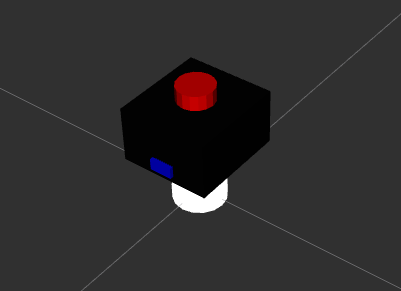
\includegraphics[scale=0.45]{obrazky-figures/robot_description_no_joint_states.png}
	\end{minipage}%
	\begin{minipage}[c]{0.5\textwidth}
		\centering
		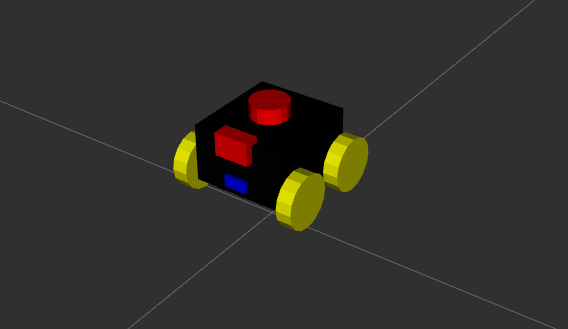
\includegraphics[scale=0.4]{obrazky-figures/robot_description_joint_states.png}
	\end{minipage}
	\caption{Zobrazení dat z robot\_state\_publisheru v nástroji RVIZ. Levý obrázek zobrazuje pouze statické tranformace (joint\_states topic je prázdný), a pravý pak celý model}
	\label{}
\end{figure}

\subsection*{Tvorba Modelu}
Jak už bylo řečeno, základní formát používaný k popisu modelů je \verb|urdf|. ROS2 využívá také druhý, rozšiřující formát \verb|xacro|. Cílem \verb|xacra| je vyřešit některé neduhy čistého \verb|urdf| a  usnadnit tak vývojářům psaní popisů robotů. Tato práce používá k popisu robota \verb|xacro| formát.

Následující blok kódu demonstruje využití téměř všech možností \verb|xacra| na jednom místě.
V čistém \verb|urdf| se velmi často opakuje téměř totožná definice \verb|link| elementu. Jedná se o zdlouhavý zápis s minimálními změnami pouze v hodnotách. Následující blok kódu vytváří makro, které umožní zkrátit tuto nepřehlednou a na chyby náchylnou sekci na jednořádkové zavolání makra. Pro zvýšení znovupoužitelnosti, využívá toto makro také parametry. Ty jsou předány v místě použití makra. Díky nim může být makro obecnější a tedy použitelné na více místech. Poslední parametr ukazuje také možnost nastavení výchozí hodnoty parametru. Parametry lze využít také v matematických výrazech. Výpočet matice setrvačnosti pro každý \verb|<link>| element je zbytečně složité a opět náchylné na chyby. Použití matematického výrazu, který se sám vyhodnotí podle hodnot předaných parametry je výrazně lepší a pohodlnější přístup.

\begin{algorithm}[h!]
	\label{}
	\caption{\textsc{Macro with params}}
	
	\DontPrintSemicolon
	\SetAlgoNoLine
	\SetAlgoNlRelativeSize{-1}
	\SetNlSty{}{}{:}
	\SetNlSkip{-1.1em}
	
	\BlankLine \Indp\Indpp
	
	\texttt{<xacro:macro name="box\_link" params="name mass x y z material:=red">}\;
	\Indp\Indp
	\texttt{<link name="\${name}">}\;
	\Indp\Indp
	\texttt{<inertial>}\;
	\Indp\Indp
	\texttt{<mass value="\${mass}" />}\;
	\texttt{<inertia ixx="\${(1/12) * mass * (y*y+z*z)}" ixy="0.0" ixz="0.0"}\;
	\Indp\Indp
	\texttt{iyy="\${(1/12) * mass * (x*x+z*z)}" iyz="0.0"}\;
	\texttt{izz="\${(1/12) * mass * (x*x+y*y)}" />}\;
	\Indm\Indm
	\Indm\Indm
	\texttt{</inertial>}\;
	\texttt{<visual>}\;
	\Indp\Indp
	\texttt{<geometry>}\;	
	\Indp\Indp
	\texttt{<box size="\${x} \${y} \${z}"/>}\;
	\Indm\Indm
	\texttt{</geometry>}\;
	\texttt{<material name="\${material}"/>}\;
	\Indm\Indm
	\texttt{</visual>}\;
    \begin{center}
	\texttt{\vdots}
	\end{center}
	
\end{algorithm}

Popis robota v \verb|xacro| formátu nelze použít jako přímou náhradu \verb|urdf|, ale musí být nejprve přeložen. K tomu slouží následující příkaz.
\begin{verbatim}
	xacro in.xacro > out.urdf
\end{verbatim}
Při překladu dojde k spojení případných více souborů dohromady, nahrazení a vyhodnocení maker, matematických výrazů a parametrů.

\section{Gazebo Simulátor}
Použití simulátoru při vývoji softwaru na řízení robotů je časté a užitečné. Umožňuje vyvíjet software i bez fyzického robota, případně testovat funkcionalitu bez vlivů reálného světa. Tato práce využívá novou \verb|ignition| větev Gazebo simulátoru. 

Před tím, než lze začít využívat výhody simulátoru, je nejprve potřeba vytvořit model robota a světy ve kterých se bude pohybovat. Nativním formátem který Gazebo využívá je \verb|sdf|. V této práci je \verb|sdf| použito k definici světů.

\subsection*{Definice světa}
Definice světů se skládá ze dvou základních částí. Nejprve se zpravidla definují obecné vlastnosti jako parametry simulace, fyzikální charakteristiky světa a pluginy. Druhou částí je pak samotná definice objektů, které se budou ve světě nacházet. Ty můžou být složené z jednoduchých tvarů, které lze definovat přímo v souboru.
\begin{verbatim}
	<box>
		<size>8 0.1 0.2</size>
	</box>
\end{verbatim}
 Druhou možností je využít \verb|<mesh>| tag pro vložení komplexnějších objektů. Umožňuje totiž vložit soubor obsahující model vytvořený například v Bleneru. Poslední možností je využití oficiální fuel knihovny, která obsahuje mnoho uživateli vytvořených modelů, které lze jednoduše vložit do světa.

\subsection*{Definice modelu}
Pro definice modelů existuje několik použitelných formátů. První možností je využít stejně jako pro světy formát \verb|sdf|. Tímto způsobem lze zapsat definici modelu ve stejném souboru jako zbytek světa. Pokud se jedná o komplexnější definici lze ji zapsat externě a vložit od stvěta pomocí \verb|<include>| tagu. Z důvodu kompatibility se zbytkem ROS2 systému umožňuje gazebo použít také \verb|urdf| potažmo \verb|xacro| soubory. Modely definované v \verb|urdf| se do světa nevkládají přímo, ale \uv{spawnují} se až po spuštění simulace. Slouží k tomu gazebo service jménem \verb|/world/world_name/create| a příkaz \verb|ign service|.

Klasický, již probraný, model definuje vizuální a fyzikální vlastnosti robota. Tato definice struktury je pro většinu nástrojů dostačující. Simulátor, který má za úkol simulovat chování robota, potřebuje dodatečné informace o tom, co jednotlivé elementy modelu reprezentují z pohledu funkcionality. K tomu slouží \verb|<gazebo>| tagy. Zde by bylo dobré zmínit, že do definic modelů lze vkládat aplikačně specifické tagy. Příkladem je právě \verb|<gazebo>|, nebo \verb|<ros2_contorl>| tag. Ostatní nástroje zpracovávající takovou definici tyto neznámé tagy ignorují.

Možným obsahem \verb|<gazebo>| tagu je buď \verb|<senzor>| nebo \verb|<plugin>|. Senzory se vždy přiřazují k nějakému existujícímu \verb|link| elementu. Tento \verb|link| pak reprezentuje fyzické vlastnosti a vzhled daného senzoru. Argumentem \verb|senzor| tagu je určení konkrétního typu snímače. V jeho těle se pak definují parametry. Ty jsou specifické pro jednotlivé typy senzorů. Gazebem podporované senzory jsou typicky komplexnější modely jako lidar a hloubkové kamery. Naopak jednodušší snímače použité na demonstračním robotovi nejsou nativně implementovány. Ultrazvukový senzor vzdálenosti je tedy ve výsledném modelu nahrazen lidarem. Aby se jeho fungování více blížilo referenčnímu senzoru, byl omezen úhel měření na 15° a počet vysílaných paprsků na tři. Modul pro sledování čáry je pak realizován pomocí tří kamer. Každá s rozlišením jeden pixel. Získanou RGB hodnotu následně zpracovává pomocný uzel.

Pluginy jsou kusy kódu, umožňující rozšířit simulátor o další funkcionalitu. Jejich použití v definici modelu slouží převážně k simulaci motorů a serv. Základní instalace Gazebo Simulátoru obsahuje mnoho užitečných pluginů. Příkladem může být \verb|DiffDrive| nebo \verb|JointController|. První zmíněný simuluje řízení robota s diferenciálním podvozkem. Druhý pak umožňuje simulovat chování podobné servu. 

\subsubsection*{ROS Gazebo Bridge}
Krása Gazebo Simulátoru je jeho provázání s ROS2 systémem. Pomocí oficiálního nástroje \verb|ros_gz_bridge| lze přemostit komunikaci mezi ROS2 systémem a Gazebo Simulátorem. Tímto způsobem lze použít stejné řídící uzly pro reálného i simulovaného robota. Gazebo vnitřně používá podobný systém topiců a zpráv jako má ROS2. Tento most pak funguje tak, že vytvoří ROS2 uzel, který zajištuje překlad mezi Gazebo a ROS2 zprávami.

Spouští se pomocí příkazu:
\begin{verbatim}
	ros2 run ros_gz_bridge parameter_bridge /topic_name@gazebo_msg_type@ignition_msg_type
\end{verbatim}
Pro efektivnější použití lze předat bridge uzlu config soubor s definicí více topiců které budou přemostěny.
\begin{verbatim}
	- ros_topic_name: "ros_chatter"
	gz_topic_name: "gz_chatter"
	ros_type_name: "std_msgs/msg/String"
	gz_type_name: "gz.msgs.StringMsg"
	direction: IGN_TO_ROS  # BIDIRECTIONAL or ROS_TO_IGN
\end{verbatim}

\subsubsection*{Zařízení kompatibility}
Ve většině případů stačí k zajištění kompatibility čisté přemostění topiců mezi Gazebem a ROSem. Ale existují také speciální případy, kdy je potřeba data nějakým způsobem upravit aby blíže odpovídaly reálnému světu. 

\begin{itemize}[leftmargin=*]
	\item{Kamera}
\end{itemize}
\vspace*{-0.5em}
Most pro přenos obrazových dat využívá na ROS2 straně zprávy typu Image. Ale jak bylo podrobněji probráno v sekci o fyzické kameře. Výstup z uzlu pro její ovládání je ve formátu CompressedImage. Data vycházející ze simulátoru musí proto být přetypovány aby byla zajištěna kompatibilita.

\begin{itemize}[leftmargin=*]
	\item{Sledování Čáry}
\end{itemize}
\vspace*{-0.5em}
Jak bylo řečeno výše, Gazebo nemá nativní podporu senzoru pro sledování čáry. Výstup ze simulátoru je tedy ve formátu tří Image zpráv, každá obsahující jeden RGB pixel. Vzhledem k tomu, že se jedná o tři samostatné zprávy, musí být nejprve seskupeny podle časových značek. Poté jsou získaná data převedena na binární hodnotu reprezentující viditelnost čáry. To je provedeno zkombinováním RGB složek pixelu na jedu grayscale hodnotu. Na ni lze jednoduše aplikovat thresholding a získat tak výsledné rozhodnutí o viditelnosti čáry.

\begin{itemize}[leftmargin=*]
	\item{Měření vzdálenosti}
\end{itemize}
\vspace*{-0.5em}
Ultrazvukový senzor je v simulátoru proveden pomocí lidaru. Je tedy potřeba zkombinovat data ze všech tří paprsků do výsledné vzdálenost. Uzel ovládající fyzický senzor, také odesílá dodatečné varování ohledně detekování překážek. Je tedy potřeba doplnit také tuto funkcionalitu.

\begin{itemize}[leftmargin=*]
	\item{Servo}
\end{itemize}
\vspace*{-0.5em}
Uzel pro ovládání fyzického serva používá action server. Tento simulovaný musí z důvodu kompatibility dělat totéž.

\begin{itemize}[leftmargin=*]
	\item{Motory, Lidar, Odometrie}
\end{itemize}
\vspace*{-0.5em}
U těchto uzlů probíhá pouze jednoduché přemapování jmen. U odometrie je rozdíl v tom, že výstupem není klasický topic ale \verb|/tf| rám.

\section{ROS2 Control}
ROS2 Control je framework implementujicí teorii řízení. V sekci o ovládání komponent byl představen uzel, který zařizuje řízení dc motorů s cílem realizovat differenciální pohyb robota. Tvorba vlastního uzlu k tomuto účelu je zcela validní přístup. Problém je v tom, že podobný uzel bude potřebovat každý mobilní robot. A proto existuje ros2 control, který má za cíl zjednodušit tvorbu řídících systémů.

\subsection{Controller Manager}
Je hlavní řídící jednotkou, která zajišťuje navázání ovladačů(controllers) a hardwarových pluginů (drivers). Manager se spouští pomocí uzlu \verb|ros2_control_node|. Jako první krok po spuštění potřebuje získat informace o robotu, kterého bude ovládat. Ty hledá v \verb|robot_description| topicu. Konkrétně z něj získá seznam kloubů a ros2 control rozhraní, kterými tyto klouby disponují. Příkazové rozhraní \verb|command_interface| slouží k posílání dat směrem k hardwaru, například nastavení rychlosti(velocity) otáčení motoru. Stavové rozhraní \verb|state_interface| pak slouží k získávání informací z dané komponenty zpět do ros2 systému, může se jednat například o výstup enkodéru motoru. Další inicializačním krokem je zpracování konfiguračního souboru. Ten obsahuje seznam použitelných ovladačů a jejich nastavení. V tento moment bude manager čekat na spuštění některého z ovladačů definovaných v konfiguračním souboru, aby mohlo dojít k jeho navázání na kompatibilní hardwarové rozhraní. Tímto krokem je vše připraveno a může započít ovládání robota.
U příkladu ovládání robota s differenciálním podvozkem je využit, již implementovaný ovladač, který zajišťuje výpočty týkající se kinematiky. Hardware plugin se pak stará pouze o ovládání motorů pomocí gpio rozhraní.

\subsection{Model}
Aby Control Manager věděl, se kterými částmi robota bude pracovat, musí být upravena \verb|urdf| definice. Konkrétně je potřeba přidat \verb|<ros2_control>| tag. V jeho obsahu je jako první vybrán konkrétní hardware plugin, který bude zajišťovat řízení komponent. Jsou zde také zapsány parametry, které budou při spuštění předány danému pluginu. Dále jsou vybrány klouby a jejich rozhraní se které bude tento plugin a potažmo ros2 control ovládat. 

\subsection{Hw Plugin}
Hardware Pluginy jak z názvu vyplývá jsou části kódu které budou v ros2 control ekosystému zajišťovat komunikaci s hardware komponentami. Narozdíl od controlerů, u kterých lze často využít existující implementace protože se požadované funkcionality často opakují. U hardware pluginů existuje mnoho různých komponent s různými rozhraními a, tak je často potřeba si napsat vlastní. Pro psaní pluginů se používá jazyk C++. Struktura jako taková je podobná lifecycle uzlům ROS2. Tato třída musí definovat speciální metody, které se volají v průběhu inicializace / destrukce objektu.

\begin{figure}[h!]
	\centering
	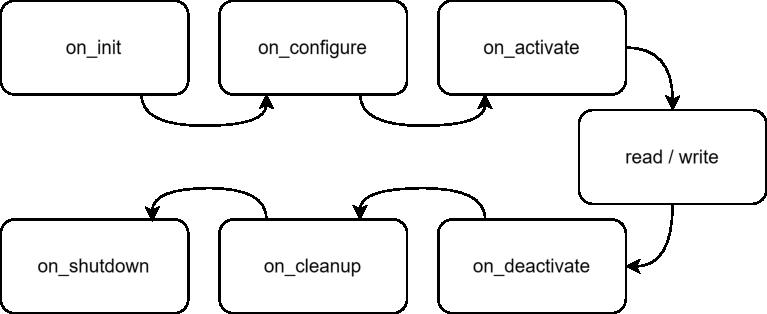
\includegraphics[scale=0.8]{obrazky-figures/ros2_control_wh_plugin_transitions.pdf}
	\caption{Základní postup volání lifecycle funkcí}
	\label{}
\end{figure}

\begin{itemize}[leftmargin=*]
	\item{\verb|on_init|}
	\vspace*{-0.5em}
	\begin{itemize}
		\item{načtení parametrů definovaných v urdf modelu}
		\item{kontrola, že klouby zadané v urdf odpovídají očekávání}
	\end{itemize}
	\item{\verb|on_configure / on_cleanup|}
	\vspace*{-0.5em}
	\begin{itemize}
		\item{připravení a nastavení hardwaru}
		\item{například nastavení gpio pinů, nastavení jejich směru, inicializace pwm}
	\end{itemize}
	\item{\verb|on_activate / on_deactivate|}
	\vspace*{-0.5em}
	\begin{itemize}
		\item{}
	\end{itemize}
	\item{\verb|export_state_interfaces| / \verb|export_command_interfaces|}
	\vspace*{-0.5em}
	\begin{itemize}
		\item{nabídne rozhraní definované v urdf a inicializované v pluginu k spárování s ovladači}
	\end{itemize}
	\item{\verb|read|}
	\vspace*{-0.5em}
	\begin{itemize}
		\item{získává hodnoty z hardwaru a ukládá je do vnitřních proměnných aby se jejich hodnoty mohly dostat k ovladačům}
	\end{itemize}
	\item{\verb|write|}
	\vspace*{-0.5em}
	\begin{itemize}
		\item{podle hodnot z vnitřních proměnných zasílá příkazy hardwarovým komponentům}
	\end{itemize}
\end{itemize}

\subsection{Controllers}
Ovladače se definují pomocí konfiguračního \verb|yaml| souboru, který následuje stejná pravidla jako konfigurace pro kterýkoli jiný ros2 uzel. Nejprve se zadávají parametry pro samotný \verb|controller_manager|. Zde se volí ovladače, které bude možné načíst. Dále pak následují konfigurace specifické pro jednotlivé ovladače.

\subsection{Integrace ros2 control s Gazebo simulátorem}
Slouží k tomu balíček \verb|gz_ros2_control|. Struktura ros2 control zůstává i pro simulátor stále stejná. Hlavní změnou je použití jiného hardware pluginu, který místo ovládání fyzické komponenty zajišťuje řízení modelu v Gazebo Simulátoru. Aby však mohl ovládat simulační prostředí musí být \verb|urdf| popis robota rozšířen o načtení dalšího Gazebo pluginu. Posledním rozdílem či zjednodušením je to, že spouštění Controller Manageru je součástí inicializace simulátoru a není tedy potřeba jej zapínat externě.

\begin{algorithm}[h!]
	\label{}
	\caption{\textsc{Plugin load}}
	
	\DontPrintSemicolon
	\SetAlgoNoLine
	\SetAlgoNlRelativeSize{-1}
	\SetNlSty{}{}{:}
	\SetNlSkip{-1.1em}
	
	\BlankLine \Indp\Indpp
	
	\texttt{<plugin filename="control-system.so" name="GazeboSimROS2ControlPlugin">}\;
	\Indp
	\texttt{<parameters>\$(find package\_name)/config/controllers.yaml</parameters>}\;
	
\end{algorithm}


\section*{Navigace a mapování}


Před zahájením mapování je nejprve potřeba vytvořit několik uzlů, které budou poskytovat informace o aktuální pozici robota, jeho struktuře a podobně.

\subsubsection*{Model}
Pro správné fungování mapování je nejprve potřeba převést reálného robota na model ve fomátu \verb|urdf|. Podrobněji se o tvorbě modelu robota mluví v %odkaz na gazebo sekci

\subsubsection*{Odometrie}
Druhým krokem k mapování a lokalizaci je získání aktuálních souřadnic, orientace a rychlosti robota. K tomu slouží odometrie. Odometrická dala lze získat několika způsoby. Jedním z často používaných a také poměrně přesných přístupů je využití dat získaných z enkodérů motorů kol a následný výpočet vzdálenosti, kterou urazily jednotlivá kola diferenciálního podvozku. Vzhledem k tomu, že použitý robot nedisponuje motory s enkodéry byl v této práci využit druhý přístup. Tím je zpracování dat získaných z imu senzoru. Integrací dat z akcelerometru a gyroskopu lze získat aktuální pozici a natočení vůči počátku. Nevýhodou tohoto přístupu je její menší přesnost a akumulace chyb vedoucí k postupnému vzdalování těchto dat od reality. Postupná akumulace chyby u odometrie vzniká u všech přístupů a ostatní části ROS2 systému realizující mapování a navigaci tak s touto skutečností počítají. V této práci tuto funkcionalitu zajišťuje uzel \verb|imu_node|, který výsledná data odesílá jako odom frame do tf subsystému. 

\begin{figure}[h!]
	\centering
	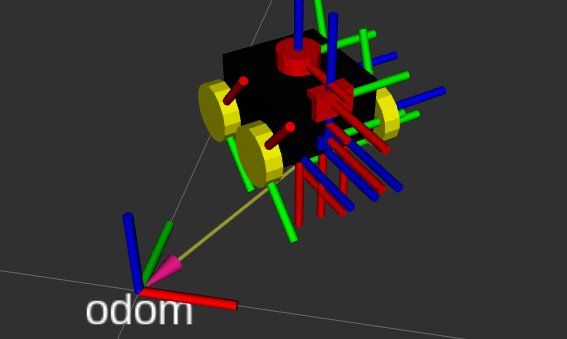
\includegraphics[scale=0.5]{obrazky-figures/odom.png}
	\caption{Zobrazení robota včetně jeho transformačních rámů v Rviz, fixed\_frame je nastaven na odom a robot se tedy může pohybovat oproti počátku souřadného systému}
	\label{}
\end{figure}

\subsubsection*{Mapování}
Posledním krokem k úspěšnému mapování je získání dat o okolním prostředí. To zajišťuje lidar senzor umístěný na robotu. Aby bylo možné data získané z lidaru správně vizualizovat v rviz musí existovat transformace mezi rámem lidaru a base frame robota. Pokud je lidar součástí definice modelu, postará se o tuto transformaci \verb|robot state publisher|.

Mapování jako takové pak zajišťuje perfektní knihovna \verb|slam_toolbox|. Jedná se o komplexní soubor nástrojů souvisejících se SLAM. Tato práce využívá \verb|async_slam_toolbox_node|. Jedná se o online, async mapování. Online znamená, že uzel pracuje nad aktuálními daty, knihovna totiž umožňuje také tvorbu mapy z před zaznamenané historie. Async pak zajišťuje zpracování vždy nejnovějších dat, což zlepšuje latenci, ale může vést k přeskočení některých scanů. Vzhledem k tomu, že slam je komplexní problém, existuje mnoho nastavitelných parametrů. Ty se předávají při spouštění pomocí konfiguračního souboru. V demo příkladech se nahází ukázkový config soubor, který byl jen s menšími modifikacemi využit i v této práci. Hlavní změnou je zvýšení rozlišení vytvářené mapy. Vývojáři knihovny předpokládají její využití v průmyslu a základní hodnoty tedy pracují s předpokladem, že robot je větší a pohybuje se ve velkých halách. Uzel pak odesílá výslednou mapu ve standardním formátu \verb|nav_msgs/OccupancyGrid| do \verb|/map| topicu.

\begin{figure}[h!]
	\centering
	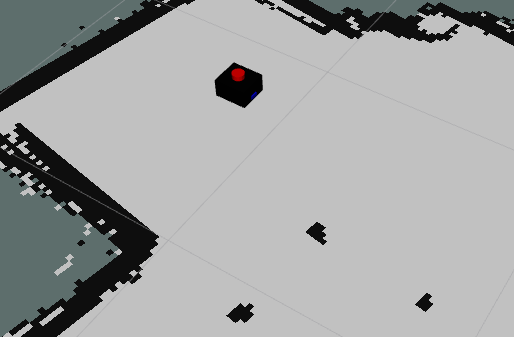
\includegraphics[scale=0.4]{obrazky-figures/slam.png}
	\caption{}
	\label{}
\end{figure}

\subsubsection*{Navigace}
Pro navigaci byla využita knihovna Navigation 2. Nav2 je v podstatě samostatný ROS2 systém skládající se z několika navzájem spolupracujících uzlů. Principiálně je Nav2 založen na behaviorálních stromech.

Z vnějšího pohledu uzly Nav2 poslouchají topicy \verb|/scan|(lidar data) \verb|map|(slam mapa) a transformace z tf systému, primárně ty související s \verb|odom| rámem. Zobrazitelným výstupem je několik costmap. Jedná se o upravenou mapu z \verb|map| topicu obohacenou o ceny jednotlivých polí. Tyto ceny jsou používány plánovacím serverem (jeden z uzlů Nav2) k určení optimální cesty k cíli. Příkaz pro zahájení navigace je přijímán action serverem se jménem \verb|/navigate_to_pose|. 

Uživatel může ovlivnit chování Nav2 systému pomocí konfiguračního souboru. Ten je poměrně komplexní a umožňuje nastavovat velké množství parametrů a dokonce vyměňovat řídící pluginy. V porovnání s slam konfigurací zde bylo potřeba změnit hodně parametrů. Protože použité motory nedokážou vyvinout menší rychlost než 0.2m/s bylo potřeba upravit minimální rychlosti. Stejně jako u slam konfigurace je robot menší a pohybuje se v menších prostorách, byly proto zmenšeny inflation vzdálenosti. Ty jsou okolo překážek a určují ceny jednotlivých polí při plánování cesty.

\begin{figure}[h!]
	\centering
	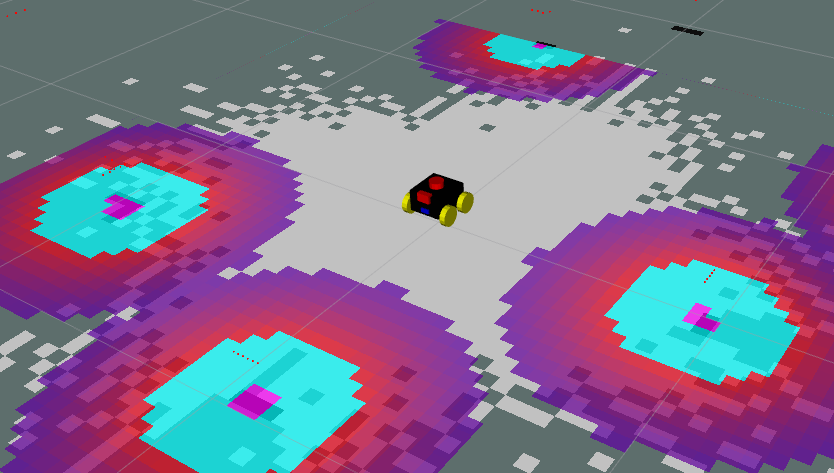
\includegraphics[scale=0.4]{obrazky-figures/nav2.png}
	\caption{}
	\label{}
\end{figure}

\section{Uživatelské rozhraní}
Uživatelské rozhraní na straně stacionárního zařízení využívá knihovnu Qt, konkrétně její python verzi PyQt5. Rozhraní jako takové je odděleno od ostatních řídících funkcionalit a pouze zajišťuje zobrazování informací získatelných z topiců a odesílání příkazů ostatním uzlům. Zbytek ROS2 systému je tedy plně ovladatelný z prostředí příkazové řádky. Co se týče implementace tak ROS2 i qt mají svůj vlastní execution loop, což vytváří problém, protože pokud jeden z nich neběží, tak daná část nefunguje. Jednou možností řešení je použití více procesů. To však vede na problémy se synchronizací. Lepší a také použitý přístup tedy je řídit oba cykly manuálně. 
\begin{verbatim}
while controllers.user_interface.global_variables.executeEventLoop:
	rclpy.spin_once(node, timeout_sec=0.001)
	app.processEvents()
\end{verbatim}
ROS2 část zajišťuje komunikaci se zbytkem systému. Obsahuje subscribery na topicy ze kterých volá qt funkce na zobrazení získaných dat. Kromě těch pak obsahuje také funkce sloužící k zasílání příkazů na servery či odesílání dat do topicků. Ty jsou volané z qt části.
Qt část se pak stará čistě o zobrazování získaných dat nebo volání ROS části v reakci na uživatelské akce.

\section{Instalace}
Výsledný systém je komplexní a obsahuje mnoho závislostí které vyžaduje pro jeho správnou funkcionalitu.

\chapter{Závěr}
Cílem práce bylo vytvořit ROS2 systém pro ovládání robota Adeept AWR 4WD a demonstrovat na něm možnosti ROS2. Tohoto cíle bylo dosaženo a implementovaný systém tak může fungovat jako ukázka možností ROS2. V rámci implementace bylo využito všech důležitých funkcionalit a konceptů používaných v ROS2. Dokumentace pak funguje jako vysvětlení jednotlivých funkcionalit případně jako rozcestník při hledání příkladu konkrétní funkcionality.

Práce pak nad rámec původního cíle demonstruje také použití dalších souvisejících nástrojů. Jedním z nich je Gazebo Simulátor, díky kterému lze jednoduše vyvíjet a testovat ROS2 uzly i bez fyzického robota. Dále pak demonstruje použití frameworku ros2\_control pro řízení motorů robota. Nakonec pak bylo hardwarové vybavení robota rozšířeno o další senzory jako IMU a lidar, které umožnili zaměřit se na problematiku mapování a navigace. V tomto ohledu byly využity nástroje slam\_toolbox a navigation2.

%Další pokračování, které bych rád uskutečnil je výměna motorů za kvalitnější, které by dysponovaly enkodéry, 
V dlouhodobějším horizontu by šlo implementovat rozšíření systému na multirobotickou aplikaci, kde by dva roboti navzájem komunikovali a společně vykonávali nějakou činnost.

%===============================================================================

% Pro kompilaci po částech (viz projekt.tex) nutno odkomentovat
%\end{document}
